% options:
% thesis=B bachelor's thesis
% thesis=M master's thesis
% czech thesis in Czech language
% slovak thesis in Slovak language
% english thesis in English language
% hidelinks remove colour boxes around hyperlinks

\documentclass[thesis=B,czech]{FITthesis}[2012/06/26]

\usepackage[utf8]{inputenc} % LaTeX source encoded as UTF-8

\usepackage{graphicx} %graphics files inclusion
% \usepackage{amsmath} %advanced maths
% \usepackage{amssymb} %additional math symbols

\usepackage{dirtree} %directory tree visualisation
\usepackage{subfig} %image side by side
\usepackage{todonotes} %todo
\usepackage{url}
\usepackage{textcomp} %degree symbol
\usepackage{color, colortbl} %color, table color
\usepackage{enumitem} %lists
\usepackage{float} %for H option in figures
\usepackage{array} %table aligment       
\usepackage{amsmath} %cases
\usepackage{svg} %svg
\usepackage{scrextend}
\usepackage{multirow}
\addtokomafont{labelinglabel}{\sffamily}



\setlength{\fboxsep}{0.005pt}
\newcommand{\tmpframe}[1]{\fbox{#1}}
%\renewcommand{\tmpframe}[1]{#1}

% % list of acronyms
% \usepackage[acronym,nonumberlist,toc,numberedsection=autolabel]{glossaries}
% \iflanguage{czech}{\renewcommand*{\acronymname}{Seznam pou{\v z}it{\' y}ch zkratek}}{}
% \makeglossaries

\newcommand{\tg}{\mathop{\mathrm{tg}}} %cesky tangens
\newcommand{\cotg}{\mathop{\mathrm{cotg}}} %cesky cotangens

\definecolor{LightCyan}{rgb}{0.88,1,1}
\definecolor{Blue}{rgb}{0.30980, 0.50588, 0.73725}
\definecolor{White}{rgb}{1, 1, 1}



% % % % % % % % % % % % % % % % % % % % % % % % % % % % % % 
% ODTUD DAL VSE ZMENTE
% % % % % % % % % % % % % % % % % % % % % % % % % % % % % % 

\department{Katedra teoretické informatiky}
\title{Detekce zboží v~ruce zákazníka pomocí analýzy snímků z~termokamery}
\authorGN{Lukáš} %(křestní) jméno (jména) autora
\authorFN{Brchl} %příjmení autora
\authorWithDegrees{Lukáš Brchl} %jméno autora včetně současných akademických titulů
\supervisor{doc. RNDr. Ing. Marcel Jiřina, Ph.D.}
\acknowledgements{Tímto bych chtěl hlavně poděkovat svému vedoucímu práce doc. Marcelu Jiřinovi za~všechny poskytnuté rady a možnost průběžných konzultací během práce. Dále pak Ing.~Jakubovi Novákovi za pomoc při řešení nesnází s~termokamerou.

Děkuji i své rodině za podporu při studiu a v neposlední řadě také děkuji Michaele Dvořákové, Ing. Iljovi Mašíkovi a Ing. Michaele Čížkové za typografické připomínky.}

\abstractCS{
Tato práce se zabývá detekcí zboží v~ruce zákazníka pomocí analýzy snímků z~termokamery. Kamera je umístěna nad regálem, kde snímá oblast bezprostředního dění před ním. Snímaná data z~kamery obsahují informace o~teplotách jednotlivých předmětů na scéně. Pomocí teplotních dat je následně možné na~snímcích segmentovat ruku a~zkoumat, zda se na scéně vyskytuje zboží. Cílem práce je průzkum možných řešení této úlohy, návrh vlastního řešení a~následně jeho implementace. V~práci je k~problému přistupováno více způsoby a je navrženo několik možných řešení. Pro snímání dat je použita termokamera FLIR A65 se sadou nástrojů eBUS SDK. Algoritmy jsou implementovány v~jazyce Java s~využitím knihovny OpenCV. Vyhodnocený algoritmus dynamického odčítání pozadí dosahuje celkové klasifikační přesnosti 88~\%.}



\abstractEN{This thesis deals with the detection of goods in the customer’s hand by analyzing images from infrared camera. The camera is located above the shelf, monitoring behavior of the customer standing in front of it. Acquired data contains informations about the temperature of the objects in the view. Using these temperature data, it is possible to segment hand and examine the presence of the goods on the scene. The aim of the thesis is to explore possible solutions of this task, to propose a solution and subsequently implement it. There are several approaches to the problem and several possible solutions are proposed. The FLIR A65 thermal camera with the eBUS SDK tool is used to capture data. The algorithms are implemented in Java using the OpenCV library. The evaluated background subtraction algorithm achieves an overall classification accuracy of 88 \%.
}
\placeForDeclarationOfAuthenticity{V~Praze}
\declarationOfAuthenticityOption{5} %volba Prohlášení (číslo 1-6)
\keywordsCS{segmentace obrazu, segmentace ruky, klasifikace, počítačové vidění, strojové učení, termokamera, FLIR, OpenCV, Java\newpage}

\keywordsEN{image segmentation, hand segmentation, classification, computer vision, machine learning, infrared camera, FLIR, OpenCV, Java}
\website{https://github.com/brchlluk/BachelorThesis} 

\begin{document}
\begin{introduction}
Rozpoznávání obrazu je bezesporu jedno z~aktuálně nejhojněji diskutovaných a~rychle se rozvíjejících témat posledních let. Prakticky denně lze sledovat nové metody a technologie tohoto oboru, které nám usnadňují práci a celkově mění náš život. Příkladem mohou být nově vznikající autonomní vozidla, která ke svému řízení využívají sadu senzorů a kamer, a mají za úkol nás co nejbezpečněji dopravit na potřebné místo. Jiným příkladem mohou být rozsáhlé neuronové sítě, které na základě vstupního obrázku zvládnou detekovat předměty, osoby a dokonce popsat činnosti, které se na snímku odehrávají. Zkrátka, oboru rozpoznávání obrazu se aktuálně věnuje velké množství lidí po celém světě a vzhledem k~tempu, jakým se všechny technologie vyvíjejí, je možné brzy očekávat převratné novinky s~užitkem pro lidstvo.

Další velmi zajímavou oblastí, která se v~posledních letech začíná značně rozšiřovat a přibližovat veřejnosti, jsou termokamery. Pomáhají nám při záchraně osob, v~průmyslu (například při monitorování nebezpečných látek), ale dokonce už i při běžných činnostech jako je hledání chyb v~tepelné izolaci našich domů.

Oblast termografie má za sebou již dlouhou řadu let výzkumu a vývoje. Zatímco infračervené záření bylo objeveno již kolem roku 1800, první prototypy kamer, které by infračervené záření zvládli zaznamenat, byly vynalezeny až kolem roku 1930. Od této doby technologie termokamer prošla několika generacemi, ale je zřejmé, že možnosti termokamer ještě nejsou zdaleka vyčerpány. Stále se objevují nové inovace a příkladem lze zmínit firmu FLIR Systems (dále jen FLIR), která je jedním z~největších výrobců termokamer na celém světě. FLIR postupně rozšiřuje své portfolio termokamer i~do neobvyklých oborů, jako jsou již zmíněná autonomní vozidla, ale snaží se zpřístupnit kamery i~pro širokou veřejnost. Jejich termografické moduly pro chytré telefony je možné pořídit za velmi lidovou cenu a jsou dostupné skoro pro každého. 

O~tom, že lidé o~obor termografie mají stále větší zájem svědčí i to, že firma FLIR v~roce 2014 představila svoji první verzi modulu pro chytré telefony a v~roce 2017  je už dostupná jeho třetí generace. V~roce 2016 byl dokonce představen i samostatný chytrý telefon s~již zabudovanou termokamerou. Je tedy zřejmé, že termokamery se velmi rychle rozšiřují do podvědomí veřejnosti a postupně se dále budou stávat již běžnou součástí dennodenních zařízení.

\begin{figure}
    \subfloat[FLIR One 3rd gen.]{{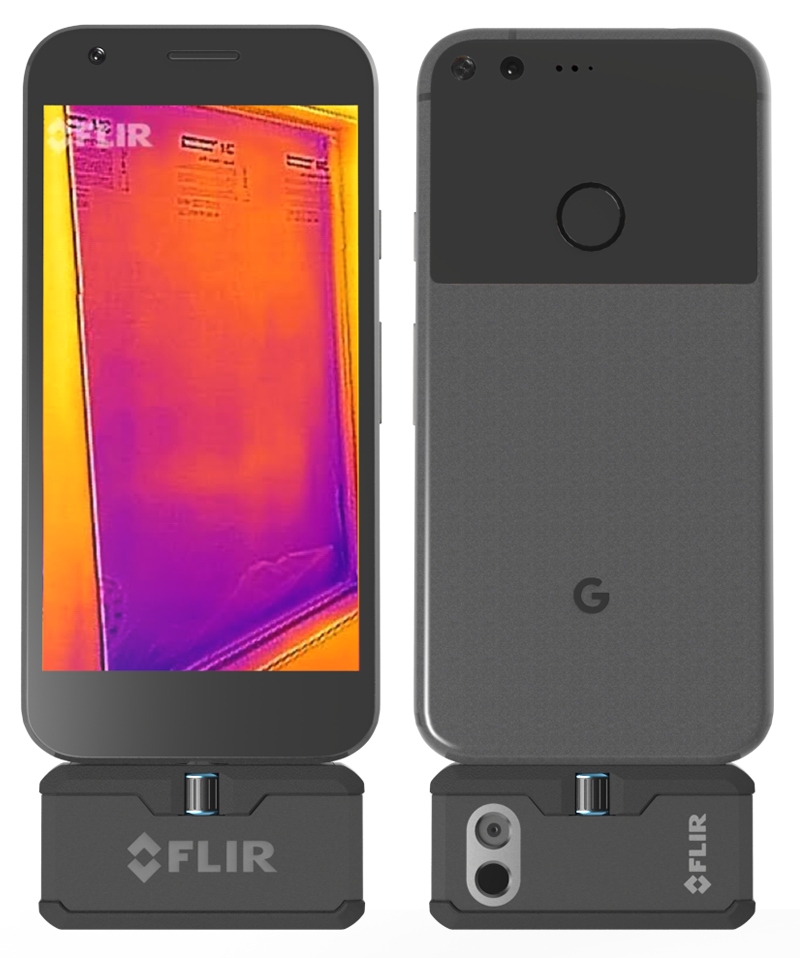
\includegraphics[width=5cm]{images/flir_one.png} }}
    \qquad
    \subfloat[CAT S60]{{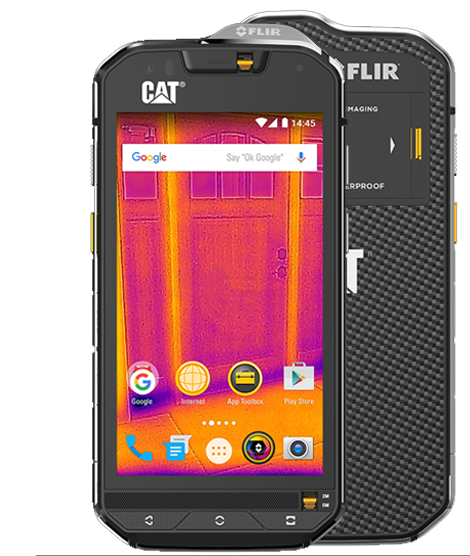
\includegraphics[width=5cm]{images/cat_s60.png} }}
    \caption{Na obrázku (a) je možné vidět přídavný modul pro chytré telefony a na (b) telefon s~již zabudovanou termokamerou}
    \label{fig:example}
\end{figure}

	\section{Motivace}
	Využití těchto nově rozvíjejících technologií by pro toto téma mělo přinést nové zajímavé objevy a poznatky k~ještě neúplně probádané oblasti. 
    
    Tématem detekce zboží v~ruce se již zabýval student Oliver Keruľ-Kmec ve své bakalářské práci \cite{kerul2016detekce}, ale bylo zjištěno, že se jedná o~poměrně náročnou úlohu. Jeho práce přináší řešení a poznatky, ale obecně je možné tvrdit, že problém ještě nebyl doposud uspokojivě vyřešen. Má tedy smysl se tématem dále zabývat a~to zejména na jiné úrovni obrazu než bylo řešeno, a tím je termografický obraz.
	
	\section{Cíl práce}
    Cílem práce je seznámení s~úlohou detekce zboží v~ruce zákazníka, prozkoumání souvisejících řešení úloh v~oblasti termokamer. Dále návrh vlastního algoritmu, který bude zboží v~ruce zákazníka schopný detekovat. Algoritmus bude implementován v~programovacím jazyku Java s~využitím volně dostupné knihovny OpenCV. Pro ověření funkčnosti algoritmu je nutné jeho vyhodnocení na vlastnoručně naměřených datech. Na základě dosažených výsledků bude provedena diskuze nad výhodami a nevýhodami využitého řešení.
    
	\section{Struktura dokumentu}
    V~první řadě je nutné obecné seznámení s~termokamerami a oblastí termografie. K~tomu slouží první kapitola, kde jsou stručně probrány důležité základy pro pochopení práce. Následně je provedena analýza zadaného problému, zavedení nutných předpokladů a představení prostředků práce. Nadcházející kapitola se pak věnuje průzkumu možných řešení a popisu navržených postupů. Ve čtvrté kapitole jsou  vyhodnoceny dosažené výsledky a pátá kapitola  je věnována  implementačním záležitostem. V~poslední části je celkové zhodnocení využitých postupů. 
    
	\section{Návaznost práce}
	Tato práce nepřímo navazuje na práci studenta Olivera Keruľ-Kmece \textit{Detekce přítomnosti zboží v~ruce zákazníka} \cite{kerul2016detekce}. 

\end{introduction}
\chapter{Termokamera}
Pro pochopení řešení této práce je nutné se seznámit s~technologií termokamer a dalšími důležitými pojmy  z~termografického oboru. Technologie a způsob použití je proti běžným kamerám rozdílná a má tedy smysl se jejím popisem zabývat.

Oblast termografie je sama o~sobě velmi náročná a mohla by být samostatným tématem rozsáhlé vědecké práce. Kapitola se věnuje pouze základním principům a pro detailnější pochopení této oblasti jsou doporučeny práce \cite{kaplan2007practical,gaussorgues2012infrared,vollmer2010infrared}.

\section{Co je to termokamera}
Termokamera je zařízení, které nám umožňuje zobrazit a zaznamenat námi jinak neviditelné infračervené záření. Podobným způsobem jako běžné kamery zaznamenávají viditelné spektrum. 

\begin{figure}[h]
  \centering
  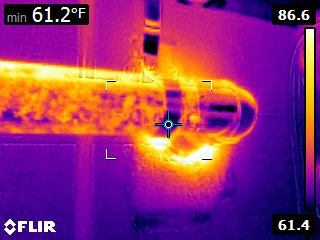
\includegraphics[width=0.7\textwidth]{images/thermal_camera_sample_image.jpg}
  \caption{Ukázkový snímek pořízený termokamerou \cite{thermalSampleImage}}
\end{figure}

\section{Princip snímání} \label{section:measurement_principle}
Snímání termokamery spočívá v~bezdotykovém měření povrchové teploty těles. Tento způsob využívá skutečnosti, že každé těleso, jehož teplota je vyšší než absolutní nula, vyzařuje tepelné záření \cite{puhl2015bezkontaktni, kadleckzadkladymereni1}. Jak se těleso stává teplejším, ve vnitřní struktuře se zrychluje pohyb atomů a molekul, a tím se tvoří více energie, kterou je potřeba vyzářit. Snímač termokamery (detektor) infračervené spektrum zaznamenává formou elektronických signálů, který jsou následně digitalizovány a převedeny na termografický snímek. 

Technologicky není možné konstruovat snímače termokamery tak, aby zachytily celý rozsah infračerveného spektra. Proto jsou vždy konstruovány pro konkrétní infračervenou oblast. V~dnešní době je to nejčastěji oblast LWIR (více o~oblastech v~\ref{sec:ir_radiation}) a to díky nižší ceně technologie a velmi dobrým výsledkům.    
    
   	\subsection{Absolutní nula}
    Absolutní nula je teoretický stav tělesa, při kterém se zastaví veškerý pohyb částic a z~tělesa již nelze odebírat žádné další teplo. Hodnota absolutní nuly je 0~kelvinů neboli -273,15 \textdegree{}C. Zatím neexistuje známý způsob, jak 0 K~dosáhnout. Jsou pouze známy způsoby a byly provedeny experimenty, které se k~dosáhnutí hodnoty absolutní nuly limitně přibližují. 
       
    \subsection{Elektromagnetické záření}
       Elektromagnetické záření je příčné postupné vlnění tvořené elektrickým a magnetickým polem. Lidé nejčastěji vnímají záření nazývané viditelné spektrum neboli světlo, které nám umožňuje vidět. Kromě viditelného spektra bylo postupem času objevováno více druhů záření, které bylo nutné rozdělit do skupin. Tyto skupiny tvoří takzvané elektromagnetické spektrum, kde jsou jednotlivá záření popsána jejich vlnovými délkami (respektive frekvencemi). Přechody mezi skupinami jsou plynulé a některé se částečně překrývají. 
       
       Záření, které lidskému oku umožňuje vidět se nazývá viditelné spektrum. Viditelné spektrum lze nalézt  mezi UV a IR zářením, a to pouze ve velmi úzkém rozsahu vlnových délek od 400 nm do 800 nm. Záření mimo viditelné spektrum je pro lidstvo nejen neviditelné, ale lidé jej nedokáží ani vnímat. Přesto je možné se zářením různých druhů dennodenně setkávat. Příkladem je ultrafialové záření, jehož zdrojem je slunce a lidský organismus ovlivňuje tvorbou kožních skvrn a přispívá na tvorbě vitamínu D. Na rozdíl od lidí však existují živočichové, kteří jsou schopni vnímat nejen viditelné spektrum, ale také UV a IR spektrum. \cite{smrvz2013bezkontaktni, kadleckzadkladymereni1} 
                   
    \begin{figure}[h]
      \centering
      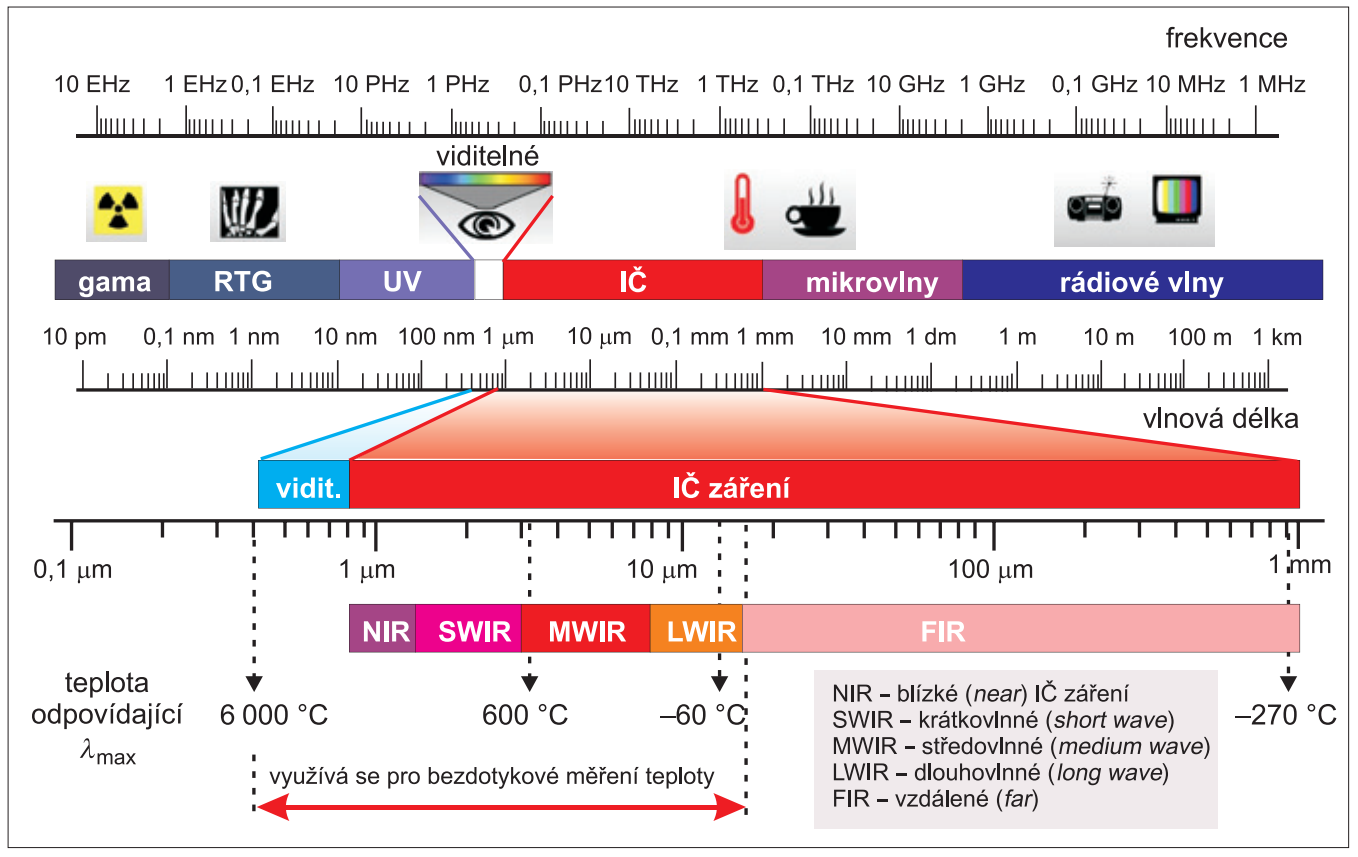
\includegraphics[width=1\textwidth]{images/elektromagneticke_spektrum.png}
      \caption{Elektromagnetické spektrum s~vyznačenými pásmy infračerveného záření 								\cite{kadleckzadkladymereni1}}
    \end{figure}
    
    \subsection{Infračervené záření} \label{sec:ir_radiation}
    Infračervené záření je pouze jedna ze skupin patřící do celku elektromagnetických záření. Jeho vlnová délka je přibližně od 760 nm do 1 mm a nachází se mezi viditelným spektrem a mikrovlnami.  \cite{stupvnankova2009ir} 
        
        Vlnová délka IR záření je závislá na teplotě tělesa, které jej vyzařuje. Obecně platí, že čím je teplota tělesa vyšší, tím se vlnová délka zkracuje \cite{kadleckzadkladymereni1}. IR záření se dále dělí na jednotlivá pásma, která však nejsou striktně daná a existuje více využívaných rozdělení \cite{stupvnankova2009ir}. Nejčastěji se však využívá obecné rozdělení uvedené v~tabulce \ref{table:ir_regions_table_common}. V~jiných zdrojích se též vyskytuje:

    \begin{itemize}[noitemsep]
      \item rozdělení dle doporučení od Mezinárodní organizace pro osvětlování (CIE),
      \item rozdělení dle normy ISO 20473,
      \item astronomické rozdělení.
    \end{itemize}

    \begin{table}[h]
      \centering
      \begin{tabular}{|c|c|c|c|}
        \hline
        \rowcolor{Blue}
        \color{White}\textbf{Název pásma} & \color{White}\textbf{Zkratka} & \color{White}\textbf{Rozsah od} & \color{White}\textbf{Rozsah do} \\ \hline
        blízké infračervené záření 	& NIR  		& 0.76 µm   & 1.4 µm   	    \\ \hline
        krátké vlnové délky   		& SWIR		& 1.4 µm 	& 3 µm		    \\ \hline
        střední vlnové délky 		& MWIR 		& 3	µm 		& 8 µm		    \\ \hline
        dlouhé vlnové délky  		& LWIR 		& 8 µm		& 15 µm		    \\ \hline
        vzdálené infračervené záření & FIR  	& 15 µm		& 1000 µm 	    \\ \hline
      \end{tabular}
      \caption{Obecné rozdělení oblastí infračerveného záření}
      \label{table:ir_regions_table_common}
    \end{table}
     
     \subsection{Absolutně černé těleso} \label{sec:absolute_black_body}
   	 Absolutní černé těleso  je ideální teoretické těleso, které pohlcuje veškeré dopadající záření všech vlnových délek. Současně s~touto vlastností se chová jako ideální zářič. To znamená, že ze všech možných těles o~stejné teplotě vyzařuje nejvíce energie. 
     
     V~reálném světě se absolutně černému tělesu blíží některé hvězdy a nebo vyrobené přístroje, pomocí kterých  jsou termokamery kalibrovány. \cite{kadleckzadkladymereni1, jakl2011experimentalni}
    
    Černé těleso si lze představit jako dutinu s~matným černým povrchem a~malým vstupním otvorem stejně jako je ilustrováno na obrázku \ref{fig:black_body_image}. Jakmile záření projde otvorem do trubky, po několika odrazech se úplně pohltí. Tedy veškeré záření, které se do absolutně černého tělesa dostane, se již zpět ven neodrazí. Pohlcené vstupní záření se přemění na energii a je zpět vysíláno pouze ve formě tepelného záření.
   
    \begin{figure}[h]
      \centering
      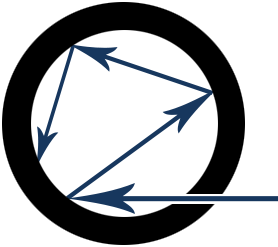
\includegraphics[width=0.3\textwidth]{images/black_body.png}
      \caption{Konceptuální černé těleso}
      \label{fig:black_body_image}
    \end{figure}    
     
\section{Konstrukce}
Všechny termokamery se skládají z~minimálně třech důležitých součástí, kterými jsou: optická soustava, detektor a obvody pro předzpracování obrazu \cite{jakl2011experimentalni,smrvz2013bezkontaktni,malik2012zpracovani}. Jednoduché schéma termokamery je možné vidět na obrázku \ref{fig:thermal_camera_scheme}. 

Základní a nejednoduší dělení termokamer je podle přítomnosti ovládacích prvků \cite{kuvzel2010bezkontaktni}. Toto dělení probíhá na:

\begin{description}[align=left]
  \item [Stacionární termokamery] obvykle využívané v~průmyslu, v~bezpečnosti, pro monitoring, apod. Stacionární kamery jsou  trvale připojeny k~počítači, který řídí jejich nastavení a přenos snímků. Obsahují pouze konektor pro připojení a nemají žádné ovládací prvky a většinou ani úložiště a baterii.
  \item [Ruční termokamery] jsou přenosné a nezávislé na počítači. Využívají se zejména pro snímkování v~terénu. Na rozdíl od stacionárních kamer obsahují vestavěnou baterii, ovládací prvky a LCD displej.
\end{description}
    
\begin{figure}[h]
  \centering
  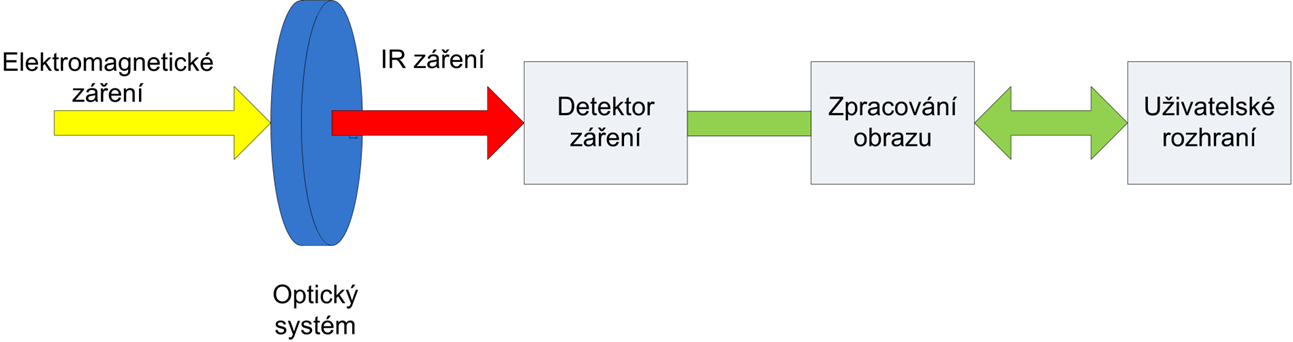
\includegraphics[width=1\textwidth]{images/konstrukce_kamery.png}
  \caption{Jednoduché schéma součástí termokamery \cite{konstrukcetermokamery}}
  \label{fig:thermal_camera_scheme}
\end{figure}
    
    \subsection{Detektor}
    Detektor  plní podobnou činnost jako snímač u~běžných RGB kamer. Na~detektor je pomocí optiky soustředěno infračervené záření, které je převáděno na elektronický signál. Signál je následně předzpracovaný korekcemi v~dalších přídavných obvodech a pak teprve převeden na výsledný snímek. Obvody pro předzpracování signálu jsou již nejčastěji součástí detektoru. \cite{smrvz2013bezkontaktni}
    
    Samotné signály z~detektoru bez aplikovaných korekcí lze zobrazit, ale výsledný obraz je velmi nekvalitní a navíc s~velkým počtem nepřesností. Pro představu je přiložen obrázek \ref{fig:flir_signal_image}, kde firma FLIR v~roce 2012 prezentovala výsledky svých nových algoritmů pro zpracování signálu z~detektoru.  Z~obrázku je patrné, že obvody pro zpracování signálu jsou velmi důležitou součástí termokamer.
    
    \begin{figure}[h]
      \centering
      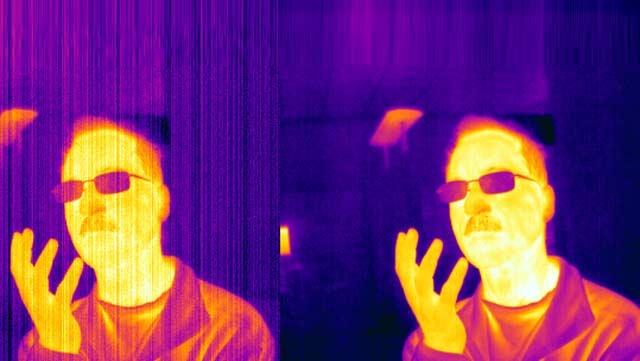
\includegraphics[width=0.6\textwidth]{images/flir_filter_with_without.jpg}
      \caption{Vlevo je snímek bez aplikovaných korekcí signálu a vpravo je snímek po aplikaci vhodných algoritmů zpracování signálu v~příslušných obvodech \cite{flirFPGAsignal}}
      \label{fig:flir_signal_image}
	\end{figure}    
    
    Termokamery lze dělit i podle druhu detektoru. Tyto dvě skupiny jsou výsledkem konstrukční technologie a jedná se o~dělení na chlazené a nechlazené detektory.
        
	\begin{description}[align=left]\label{description:detector_types}
      \item [Chlazené detektory,] někdy též označovány jako kvantové, přináší velmi přesné měření teplot, vysokorychlostní snímání, řádkové snímání (až 62~000 FPS v~případě \cite{flirSc7000}) a lepší zpracování šumu. V~závislosti na materiálu detektoru lze přizpůsobit pro IR oblasti SWIR, MWIR a LWIR. Kvůli nutnému chlazení mají větší rozměry a jejich váha se pohybuje v~jednotkách kg. Nevýhodou je několikanásobně vyšší cena oproti nechlazeným detektorům.
      \item [Nechlazené detektory] jsou konstrukčně jednodušší, spolehlivější, mají menší energetickou spotřebu a jsou cenově dostupné veřejnosti. V~dnešní době jsou nejčastější nechlazené detektory na bázi mikrobolometrů. Zajímavostí je fakt, že se dá dosáhnout velmi kompaktních rozměrů. Například detektory FLIR řady Lepton mají rozměry přibližně 1 $\times$ 1 $\times$ 0.7 cm. Tyto detektory se pouze ojediněle objevují pro jinou IR oblast než je LWIR. Nevýhody nechlazených detektorů jsou méně kvalitní výstup a~menší přesnost měření oproti chlazeným detektorům.
    \end{description}
        
    Chlazené detektory jsou velmi specifickou záležitostí, týkající se převážně extrémních využití (záchranné a bezpečnostní složky, armáda, vědecké a výzkumné ústavy, apod.), jejich popis a bližší informace nebudou součástí této práce. Podrobné detaily o~těchto detektorech lze nalézt v~knihách \cite{daniels2010field, rogalski2010infrared}.
        
    Naopak s~nechlazenými detektory je možné se setkat téměř ve všech běžných případech. Technologie nechlazených detektorů využívá výhradně mikrobolometrického pole \cite{vojavcekco, jakl2011experimentalni}. Toto dvourozměrné pole je složeno z~miniaturních bolometrů, které jsou citlivé na dopadající infračervené záření. Jednotlivé bolometry mění své elektrické odpory v~závislosti na množství tepelného záření snímaného tělesa. Každý odpor znamená jednu hodnotu signálu a jeden výsledný pixel obrazu. Rozlišení nechlazených detektorů je dáno počtem uspořádaných bolometrů v~matici. 
    
    \begin{figure}[h]
      \centering
      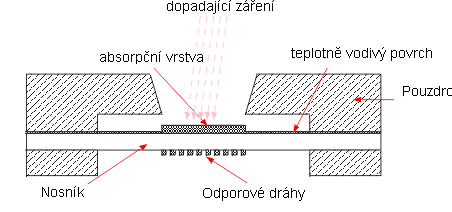
\includegraphics[width=0.6\textwidth]{images/bolometer_scheme.png}
      \caption{Schéma bolometru \cite{vojavcekco}}
      \label{fig:bolometer_scheme}
	\end{figure}  
    
    Rozlišení termokamer se obecně v~porovnání s~RGB kamerami pohybuje na skromnějších hodnotách. Od dnešních nejnižších rozlišení 80 $\times$ 60 pixelů až po extrémní třídu s~1024 $\times$ 1024 pixely. Je to z~toho důvodu, že pro dosažení dvojnásobného rozlišení termokamery,  je nutné čtyřnásobné zvětšení počtu bolometrů v~matici.
    
	\subsection{Optická soustava}
     Termokamery nemohou využívat běžnou optiku ze skla, tak jako ji využívají klasické kamery. Je to z~toho důvodu, že běžná optika infračervené záření převážně odráží než propouští. V~dnešní době již existuje více druhů používaných materiálů pro objektivy termokamer, ale nejčastěji se využívá germánium nebo jeho slitina.  \cite{kadlecsovatermokamery,stupvnankova2009ir}
     
     Optika z~germánia slouží také jako filtr všech ostatních vlnových délek a~k~samotnému detektoru, v~případě germánia, se dostává pouze záření z~pásma LWIR nebo MWIR (v~závislosti na úpravách optiky). Na optice jsou dále naneseny antireflexní nano vrstvy pro zvýšení propustnosti infračerveného záření. Optika a nano vrstvy termokamer jsou velmi šetrné a neodborným zacházením mohou být způsobena nevratná poškození. 
     
     Optika bohužel přichází o~své vlastnosti i postupem času. Jedná se zejména o~vnější vlivy, které způsobují její oxidaci a tím snižují propustnost infračerveného záření. Více o~volbách optických materiálů a jejich porovnání lze nalézt v~článku \cite{vandervlugtchoosing}.
     
\section{Specifikace a parametry}\label{sec:thermal_camera_features}
Seznam důležitých parametrů ovlivňující klíčovou funkčnost a možnosti termokamer jsou uvedeny v~tabulce \ref{table:thermal_camera_features}. K~jednotlivým parametrům je vždy uveden příklad a vysvětlující komentář.
    
\begin{table}[h]
	\centering
    \begin{tabular}{|p{4.5cm}|p{3cm}|p{6cm}|}
      \hline
      \rowcolor{Blue}
      \color{White}\textbf{Parametr} & \color{White}\textbf{Příklady} & \color{White}\textbf{Komentář}   \\ \hline
      Rozlišení detektoru & 240 $\times$ 180 pixelů &  Obecně platí, že vyšší je lepší. \\  \hline
      Typ detektoru & nechlazený FPA & Chlazený (kvantový) nebo nechlazený, více v~\ref{description:detector_types}.\\  \hline
      Snímané spektrum & LWIR, MWIR & Snímaná část IR spektra, více v~\ref{sec:ir_radiation}. \\ \hline
      Obnovovací frekvence & 30 Hz &  Počet snímků, které je kamera schopna za vteřinu pořídit. \\ \hline
      Rozsah měřených teplot & 0 - 320 \textdegree{}C & Často více možných voleb v~souvislosti s~režimem kamery \\ \hline
      Úhel záběru & 20\textdegree{} $\times$ 25\textdegree{} & Často uváděná také ohnisková vzdálenost \\ \hline
      Citlivost (NETD) & 50 K, 0.05 \textdegree{}C & Vyjadřuje, jaké nejmenší teplotní rozdíly je na povrchu černého tělesa termokamera schopna zaznamenat. \\ \hline
      Přesnost &  $\pm$ 5 \textdegree{}C nebo 5 \% & Chyba, se kterou je nutné počítat při interpretaci výsledků. Platí horší údaj. \\ \hline
      Formát zaznamenávaných snímků & 14 bit MONO, 14 bit linear  & Výsledný interpretovatelný formát a~bitová kvalita. \\ \hline
      Provozní teplota & -10 - 50 \textdegree{}C & Důležitý údaj pro využití v~nepokojových podmínkách.\\ \hline
      Komunikační standardy & GenICam, GigE &  V~dnešní době již výhradně protokol GenICam s~jedním z~přenosových standardů. \\  \hline
    \end{tabular}
    \caption{Klíčové parametry při volbě termokamery.}
    \label{table:thermal_camera_features}
\end{table}
    
    \subsection{Aklimatizace kamery}
     Aklimatizace kamery znamená dobu ustálení, kterou termokamera potřebuje, aby zaznamenávala co nejpřesnější výsledky. V~praxi to znamená stabilizování teploty detektoru na předem danou hodnotu, běžně kolem 30 \textdegree{}C u~nechlazených detektorů. Dostat se a udržovat stabilní teplotu detektoru má na starosti speciální vnitřní obvod. Tento údaj u~některých termokamer není uvedený a~přitom se dá považovat za velmi důležitý.

\section{Získávání dat} \label{section:retrieving_camera_data}
Práce se stacionární termokamerou probíhá o~něco složitějším způsobem než je proti ručním kamerám zvykem. Kamera nemá žádné interní úložiště, display ani ovládací prvky. Všechna práce, jako je ovládání kamery a~získávání dat, probíhá pomocí síťového rozhraní a je řízena počítačem. \cite{kuvzel2010bezkontaktni}

Uvedené informace v~této části, se týkají primárně kamery FLIR řady Ax5 využité v~této práci, ale obecně je lze aplikovat na všechny stacionární kamery využívající standardy GenICam a GigE Vision. Tato rozhraní jsou běžně využívány nejen u~termokamer od výrobce FLIR, ale i u~zařízení ostatních výrobců.
    
    \subsection{GigE Vision}\label{section:gige_vision}
    Standard GigE Vision byl v~roce 2006 vytvořen pro potřeby vysoce výkoných průmyslových kamer. U~jeho vzniku stálo celkem 12 firem a nyní je spravován asociací AIA. GigE Vision definuje protokol pro vysokorychlostní přenos obrazu a komunikaci s~kamerami. Jeho úkolem bylo unifikovat stávající protokoly pro průmyslové kamery a umožnit lepší kompatibilitu hardwaru a softwaru. Architektura GigE Vision vychází ze standardního internetového protokolu UDP, takže je možné kamery používat v~běžné síťově infrastruktuře. \cite{aiaGigeVision} 

    \subsection{GenICam}\label{section:genicam}
    Standard GenICam byl v~roce 2006 vytvořen sdružením EMVA. Jednalo se primárně o~snahu vytvoření univerzálního programového rozhraní pro průmyslové kamery strojového vidění. U~zařízení s~podporou GenICamu tedy z~hlediska vývoje nezáleží na technologii přenosu, vlastnostech kamery, typu kamery a~dokonce ani na výrobci kamery. Kamery mohou být připojeny přes rozhraní GigE Vision, USB3 Vision a přesto jsou způsoby konfigurace, snímání, atd. díky jednotnému rozhraní vždy stejné. \cite{emvaGenicam} 
    
    K~tomu, aby vše správně fungovalo a bylo možné standard dále rozšiřovat, je GenICam rozdělen do několika nezávislých modulů, které jsou dále popsány přímo na stránkách výrobce. Stejně tak lze na stránkách sdružení EMA nalézt referenční implementaci pod BSD licencí. Standard se dále vyvíjí a rozšiřuje s~pomocí požadavků uživatelů.

    \begin{figure}[h]
      \centering
      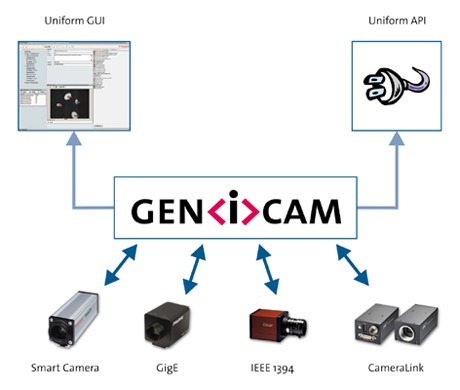
\includegraphics[width=0.8\textwidth]{images/genicam_protocol.jpg}
      \caption{Koncept GenICam protokolu \cite{genicamProtocolImage}}
      \label{fig:genicam_protocol}
	\end{figure}      
    
    \subsection{Dostupný software}
       Existují již hotové programy pro práci se stacionárními termokamerami, ale i~v ~placených verzích těchto softwarů nelze nalézt všechna potřebné nastavení a funkce. Je to z~toho důvodu, že tyto softwary jsou většinou pro průmyslové aplikace jako je monitoring, tvorbu reportů a ostatní komerční činnosti. 
       
       Příkladem je placený software FLIR Tools+ \cite{flirtools} přímo od výrobců termokamer FLIR. Tento software podporuje přenos obrazu z~kamery a jeho následné zobrazení, ale snímky jsou přenášeny pouze v~8-bitovém formátu. Dále nedovoluje ukládání surových dat, nepodporuje kontinuální ukládání a~ani zásah do nastavení kamery. 
       
       Všechny nalezené alternativní softwary mají též velmi omezené možnosti a~funkce. Kvůli tomu je vhodné využít SDK a zabývat se tvorbou vlastní aplikace pro ovládání kamery a získání snímku pro nutné potřeby řešení této práce. 
    
    \subsection{Sada vývojových nástrojů}\label{section:sdk}
    Lepším řešením, ale bohužel časově náročnějším, je využít vhodnou sadu vývojových nástrojů (SDK) a s~kamerou pracovat na úrovni kódu. Kamera FLIR A65 podporuje rozhraní GigE a GenICam a ač byly oba standardy vytvořeny již v~roce 2006, dostupných SDK je v~řádu jednotek. Nejčastěji využívané jsou:
      
    \begin{itemize}[noitemsep]
    \item Atlas SDK \cite{atlasSdk},
    \item JAI SDK \cite{jaiSdk},
    \item ActiveGigE \cite{activeGige},
    \item eBUS SDK \cite{ebusSdk}.
    \end{itemize}
      
    Všechny výše uvedené SDK podporují standardy GigE Vision a GenICam. Liší se použitým programovacím jazykem, kvalitou dokumentace, množstvím ukázkových programů a také dostupností. Stručně shrnuto:
    
    \begin{description}[align=left]
	\item [Atlas SDK] je dostupné pouze k~zakoupeným kamerám značky FLIR. Práce s~Atlas SDK probíhá v~jazyce C\# nebo prostředí MATLABu. Práce s~Atlas SDK je velmi snadná, má velmi dobrou dokumentaci a ukázkové kódy. Jedinou nevýhodou je omezený přístup k~nastavování jednotlivých parametrů protokolu.
    \item [JAI SDK] je produkt od výrobců průmyslových kamer JAI. V~současné době se firma JAI podílí také na rozvíjení standardů GigE Vision a GenICam. Jejich SDK je možné využívat v~jazyce C/C++ nebo v~C\#. Je zdarma, obsahuje velmi detailní dokumentaci a dostatečné množství ukázkových kódů. Součástí SDK je ovladač Filter driver pro urychlení přenosu dat. 
    \item [ActiveGigE] je SDK firmy A\&B Software. Na rozdíl od jiných SDK ho lze využít ve spoustě různých prostředích a programovacích jazycích. Je dostupné pro: Visual Studio, Visual Basic (VB), Delphi, PowerBuilder, Java, Matlab, Python, QT, Adobe Flash, LabView, GE Fanuc, Indusoft Studio. Zajímavou záležitostí je vkládání ActiveGigE objektů přímo do programů od Microsoftu (Word, PowerPoint) s~možností přenosu reálného obrazu. Ze všech porovnávaných SDK obsahuje v~základu nejvíce implementovaných funkcí. Samozřejmostí je rozsáhlá dokumentace a~ukázkové kódy. Jedinou nevýhodou se zdá být cena, ta je k~dubnu 2017 stanovena na 495 dolarů za licenci.
    \item [eBUS SDK] je od firmy Pleora, která se stejně jako JAI podílí na rozvíjení standardů pro strojové vidění. Je dostupné jak pro jazyk C/C++, tak pro C\#. Jeho použití je díky rozsáhlé dokumentaci a ukázkovým zdrojovým kódům velmi snadné. Součástí eBUS SDK je také ovladač Universal Pro Driver pro zvýšení propustnosti síťového rozhraní a snížení zátěže. eBUS SDK je pro kamery FLIR dostupné zdarma, pro kamery ostatních výrobců je licence zpoplatněna.
    \end{description}
    



\chapter{Analýza}
V~této kapitole jsou popsány existující řešení úlohy detekce zboží v~ruce a~následně zmíněny zajímavé související práce týkající se termokamery. Poté je proveden rozbor zadané úlohy a stanovení nutných předpokladů pro řešitelnost. Dále jsou popsány přínosy, které termokamera v~řešení tohoto problému poskytuje a následně i překážky se kterými je nutno počítat. V~poslední části jsou představeny dostupné hardwarové a softwarové prostředky.

\section{Současný stav řešení problematiky} 
Nebyly nalezeny žádné dostupné informace o~tom, že by se problematikou zboží v~ruce zákazníka ve světě někdo zabýval. Jediné dostupné řešení lze nalézt právě u~studenta Olivera Keruľ-Kmece v~jeho bakalářské práci \cite{kerul2016detekce}, který problém řešil s~jinou technologií než se zabývá tato práce. Řešený problém je tedy stejný, ale díky rozdílnosti technologií je k~němu nutné navrhnout nové postupy a~metody.

V~jeho řešení je využita kamera Microsoft Kinect, která současně snímá klasický RGB obraz a zároveň k~tomu hloubkovou mapu. Jeho řešení využívá dva různé klasifikátory. Vstupem prvního klasifikátoru je segmentovaný záběr ruky pomocí hloubkové mapy. Na tomto vstupu se vypočítá 60 předem daných příznaků a následně je ke klasifikaci využit klasifikátor Gradient boosted trees. Druhý klasifikátor je využit ke zvýšení přesnosti algoritmu a~klasifikuje posloupnost tříd, která je získaná prvním klasifikátorem. Posloupnosti jsou rozděleny pomocí algoritmu SIFT na vložení ruky a vyjmutí ruky z~regálu.

	\subsection{Související práce s~termokamerou}
    Existuje samozřejmě velké množství prací, které se zabývají segmentací termografických snímků a detekcí objektů, ale jsou vybrány jen ty nejzajímavější, které byly nalezeny. \todo{}Nejčastěji lze nalézt práce, které se zabývají detekcí obličeje nebo detekcí gest.
    
    První z~těchto prací je \cite{saba2012dante}, která se zabývá detekcí ruky a sledování její trajektorie s~využitím termokamery a kamery Microsoft Kinect. V~uvedené práci jsou přijímány dva obrazové zdroje a to hloubková mapa a termovizní snímek. Kamery mají rozdílnou optiku, takže je nutné jednotlivé snímky perspektivně upravit. K~tomu je využita knihovna OpenCV a transformační matice homografie, která slouží pro převod mezi jednotlivými snímky. V~uvedené práci bohužel není ani zmínka o~synchronizaci kamer, která se následně v~této práci ukázala jako velký problém.
    
    V~uvedené práci je následně využito dynamického odčítání pozadí \cite{opencvMOG}, pomocí kterého je na snímcích získáno popředí. Na termovizním snímku je dále aplikováno Otsu prahování \cite{otsu1975threshold} pro získání ruky, na které jsou vypočítány konvexní body pro získání prstů. Na snímku ruky jsou pak získány atributy, které se týkají primárně teplot a snímek je klasifikován pomocí klasifikátoru SVM. 
    
    Dvě různé kamery a metoda dynamického odčítání pozadí je využita také v~práci \cite{zeng2012hand} pro detekci gest. Zarovnání dvou obrazových zdrojů je též řešeno pomocí matice homografie a synchronizace není zmíněna. Segmentace probíhá pouze formou odečtení pozadí, podle teplot se nesegmentuje. Po tomto kroku už se na snímek jen aplikují morfologické operace a následně je na snímku vyhledána ruka.
    
		Další zajímavou prací je \cite{appenrodt2010data}, kde se autor zaměřuje na detekci gest a porovnává při jednotlivé využité zdroje obrazu a to: klasický RGB, hloubkovou mapu, termovizní snímek. Následně je provedena segmentace ruky na termovizním snímku pomocí binárního prahování a tento obraz je sloučen s~nejbližšími oblastmi hloubkového obrazu. Na tomto obraze jsou dále získané atributy a snímek je klasifikován pomocí Hidden Markov Models (HMM).

Přínosná je též práce \cite{duarte2014segmentation}, kde jsou popsány běžné způsoby pro segmentaci termovizních snímků, který pak byly vyzkoušeny při řešení této práce.


Často lze objevit \cite{sato2000fast} informaci o~tom, že se počítá s~tím, že teplota ruky se pohybuje v~určitém běžném rozsahu a lze segmentovat podle teplot s~pomocí binárního prahování. Tento jednoduchý způsob se následně osvědčil i v~této práci.

\section{Analýza zadaného problému}
Zadání problému je vcelku přímočaré. Pro vstupní snímek je nutné rozhodnout, zda se na něm nachází ruka nebo ruka se zbožím a nebo se na něm nenachází nic zajímavého. Je však potřeba počítat s~tím, že se nejedná pouze o~návrh algoritmu, ale také o~získání samotných dat a v~neposlední řadě také ověření správného postupu vyhodnocením. 

Prvním nezbytným krokem je tedy zaměřit se na to, jakým způsobem budou data získávána. V~\ref{section:retrieving_camera_data} byly popsány možné metody získání dat, ze kterých plyne, že běžně dostupné softwary jsou pro tuto úlohu nedostačující. Je tedy nutné poohlédnout se po vhodném SDK, seznámit se s~jeho rozhraním a~vytvořit aplikaci pro kontinuální ukládání surových dat. Přijímaná data z~kamery není vhodné převádět do komprimovaného formátu z~důvodu zachování maximální kvality.

Dalším nutným krokem je průzkum nasnímaných dat a navržení vhodného postupu jejich předzpracování. Tento postup by měl data zejména omezit na určitou oblast zájmu a převést do normalizovaného rozsahu teplot. Podle nutnosti pak záběr patřičně upravit a nakonec redukovat šum.

Na předzpracované snímky aplikovat vhodné algoritmy a tím získat potřebné informace k~dalšímu rozhodování o~výsledku. S~přihlédnutím k~faktu, že zboží má nižší teplotu než ruka, by zboží mělo být ve většině případech rozlišitelným. Otázkou zůstává, jak velké předměty je ještě možné detekovat než je dosaženo možností algoritmu a limitu termokamery. S~limitem termokamery bude souviset generovaný šum detektoru, se kterým je nutné se vypořádat. 

Posledním krokem je klasifikace do předem definovaných tříd. Tyto třídy by mohly být tři a to: pozadí, ruka, ruka se zbožím. Vzhledem k~tomu, že určit pozadí lze triviálním způsobem, bude brána v~úvahu pouze binární klasifikace třídy ruka a ruka se zbožím.

Je zřejmé, že zboží které na~snímku není vidět, například je schované v~dlani ruky, nelze tímto způsobem detekovat. V~práci se tedy berou v~potaz pouze snímky, kde zboží viditelné je. V~práci se též neřeší o~jaký typ zboží se jedná, protože to se samotnou termokamerou není zjistitelné a~existují k~tomu lepší metody. 

\section{Nutné předpoklady}
Aby byl problém termokamerou řešitelný, musí být bráno v~potaz několik předpokladů, které souvisí s~teplotou snímaných objektů. Uvedené předpoklady pouze vylučují extrémní případy, které se běžně ve vnitřních prostředí nestávají, ale je nutné je brát na vědomí.

	\subsection{Předpoklad pro teplotu ruky na snímku}\label{section:hand_temp_prereq}
	O~termoregulaci se v~lidském těle stará část mozku s~názvem hypothalamus.  Povrchová teplota lidského těla není stabilní a v~některých situacích se znatelně mění, zato teplota lidského jádra zůstává dlouhodobě neměnná a to dokonce i v~případě velkých výkyvů okolních teplot. \cite{pvrikopa2011navrhnvete}
    
    Průměrná teplota zdravého člověka na povrchu čela je při běžných pokojových podmínkách 36 - 37 \textdegree{}C \cite{mlvcak2007mapovani}. Končetiny, a zvláště prsty, jsou vždy o~něco chladnější, protože krev nejdříve putuje přes životně důležité orgány a až poté se dostává do končetin. Rozvádění krve až do končetin je pro tělo náročné, a~v~rámci vlastních experimentálních měření bylo zjištěno, že při přechodu z~chladnějších venkovních podmínek do pokojové teploty je povrchová teplota ruky schopna klesnout i o~10 \textdegree{}C níž, než je její běžný stav. Tento pokles trvá několik minut, dokud se tělo neaklimatizuje.
    
    V~této práci se tedy počítá s~tím, že snímaný člověk se již nějakou dobu pohyboval v~běžné pokojové teplotě a teplota jeho ruky se již ustálila.
    
    \subsection{Předpoklad pro teplotu zboží a regálu na snímku}
    Regál je umístěn v~místnosti s~pokojovou teplotou a jednotlivé zboží má velmi podobnou teplotu jako je teplota vzduchu v~místnosti. Teplota zboží v~regále musí být rozlišitelná od ruky, jinak by úloha termokamerou nebyla řešitelná.
    
    \subsection{Předpoklad pro teplotu podlahy na snímku}
    Pomocí vlastních experimentálních měření bylo zjištěno,že podlaha běžné místnosti je ve většině případů o~pár desetin stupňů Celsia studenější než je teplota vzduchu v~místnosti. V~práci se počítá s~tím, že teplota podlahy nepřevyšuje teplotu zboží a tedy ani ruky na snímku.
    
\section{Výhody využití termokamery pro tuto úlohu}
Tato úloha lze samozřejmě řešit i pomocí jakékoliv barevné kamery. Například způsobem, který je uveden v~již zmíněné práci Olivera \cite{kerul2016detekce}. Všechna řešení pomocí klasické barevné kamery by k~segmentaci ruky nejčastěji využívaly její barvu. Barva kůže není přirozeně nikde definovaná a navíc je závislá na světelných podmínkách v~dané místnosti. Tento způsob segmentace tedy nemusí vždy fungovat naprosto korektně a obecně není moc dobré se na barvu kůže zcela spoléhat. Dalším možným problémem je případ, kdy má zboží podobnou barvu jako ruka, což je díky různorodosti zboží běžný případ. 

V~\ref{section:hand_temp_prereq} bylo zjištěno, že teplota ruky je silně ovlivněna působením chladného vnějšího vlivu. Tento případ je ale v~reálném světě prostředí úlohy velmi málo pravděpodobný, protože člověk se ve vnitřním prostředí často velmi rychle aklimatizuje. Pokud by přeci jen tento případ opravdu nastal a~teplota ruky klesla například z~běžných 35 \textdegree{}C na 25 \textdegree{}C, byla by stále rozlišitelná od zboží, které dosahuje pokojové teploty někde mezi 16 až 22 \textdegree{}C. Řešení s~termokamerou by tedy mělo být pro segmentaci ruky robustnější, než segmentování ruky podle barvy s~běžnou RGB kamerou.

Další výhodou je, že termokamera není závislá na světelných podmínkách. Snímá totiž pouze námi neviditelné infračervené záření (\ref{section:measurement_principle}). Z~toho plyne, že stejné výsledky lze naměřit i v~úplné tmě.

Posledním zajímavým poznatkem je, že snímání termokamery neovlivňují barvy ani vzory, takže výsledný obraz obsahuje méně rušivých elementů než například běžný RGB obraz.

\section{Překážky při snímkování s~termokamerou}
Pří snímkování s~termokamerou je nutné brát v~potaz několik skutečností, které ovlivňují snímaná data a mohou též vést k~chybným výsledkům měření. Tyto skutečnosti mohou být dané konstrukčními vlastnostmi kamery a nebo se  jedná o~uživatelské chyby nastavení.

	\subsection{Korekce signálů detektoru - NUC}\label{section:nuc}
    Tak jako běžné kamery i termokamera se při snímkování zahřívá. Změna teploty detektoru pak ovlivňuje jednotlivé mikrobolometry a to tím, že začne vznikat posun hodnot signálů (temperature drift). Tento posun zvládne kamera do určité míry kompenzovat interní logikou, ale když už posun překročí jistý limit, je automaticky spuštěna kalibrační funkce NUC neboli Non-Uniformity Correction. Termokamera vloží mezi objektiv a detektor na krátký okamžik závěrku, která simuluje jednotné homogenní prostředí. S~pomocí tohoto uniformního prostředí jsou nastaveny korekce pro normalizaci hodnot signálů. 
    
    V~době kalibrace termokamera nepřenáší obraz. Tato kalibrace trvá přibližně vteřinu a její četnost je v~závislosti na změnách teploty detektoru. Kalibraci NUC tedy může spustit i změna teploty prostředí. Z~počátku měření se NUC provádí ve velmi krátkých časových intervalech, ale jak se teplota detektoru stabilizuje, provádí se NUC již méně častěji.
    
   	Více informací o~NUC a obecně o~problému posunu signálů bolometrů se lze dočíst v~\cite{olbrycht2014new, riou2004nonuniformity}.
    
    \subsection{Přenos snímků}\label{section:transmissio_errors}
    Protokol GigE pro přenos snímku z~kamery vychází z~internetového protokolu UDP (User datagram protocol \cite{postel1980user}). To znamená, že na rozdíl od TCP (Transmission Control Protocol \cite{postel1981transmission}) protokolu odesílatel neověřuje, zda příjemce data obdržel. Může se tedy stát, že některé snímky nemusí být vůbec přijaty. Jedná se spíše o~výjimečný případ, ale přesto je potřeba s~touto skutečností počítat. 
    
  	\subsection{Vady optiky}\label{section:lens_deffects}
    Optika termokamery není, tak jako žádná optika, dokonalá. Objevují se zde optické vady stejně jako u~tradičních objektivů pro běžné kamery. Obecně lze říct, že maximální obrazovou kvalitu lze nalézt v~oblasti, která je co nejblíže středu obrazového pole. V~těchto místech je obraz nejostřejší, nezkreslený a~s~největší rozlišovací schopností. 
    
    Na obrázku \ref{fig:camera_2_lens_deffects} je zobrazen neupravený snímek neutrálního prostředí, kde je možné pozorovat optické vady termokamery FLIR A65 s~ohniskovou vzdáleností 25 mm. Z~obrázku je zřejmé, že největším problémem je vinětace v~rozích, která velmi výrazně ovlivňuje výsledné teploty v~této oblasti.
     
    \begin{figure}[h]
      \centering
      
\includegraphics[width=1\textwidth]{images/camera_2_lens_deffects.jpg}
      \caption{Ukázkový snímek optických vad u~termokamery  FLIR A65 s~ohniskovou vzdáleností 25 mm}
      \label{fig:camera_2_lens_deffects}
    \end{figure}  

	\subsection{Chyby měření a vyhodnocování}
    Při snímání s~termokamerou mohou chyby vznikat už při měření a to zejména chybným nastavením kamery. Kamera na základě těchto chybných nastavení stanovuje neodpovídající teploty. Tyto parametry jsou například: emisivita, zdánlivě odražená teplota a atmosferické vlivy. V~rámci práce je nutné teploty od sebe umět rozlišit, ale není nutné znát jejich přesné hodnoty. Proto se nastavení těchto parametrů explicitně nezmiňuje a pro účely této práce nejsou klíčové. Vliv těchto parametrů a postupy, jak je správně nastavit, lze nalézt v~literatuře \cite{flirA65Spec,puhl2015bezkontaktni,smrvz2013bezkontaktni,kuvzel2010bezkontaktni}.

\section{Dostupné prostředky}
V~této části jsou popsány hardwarové a softwarové prostředky, které jsou v~rámci práce dostupné.

	\subsection{Dostupná technika}\label{sec:used_equip}
 	V~práci byly v~průběhu využity nezávisle dvě termokamery FLIR A65. Kamery se od sebe lišily ohniskovou vzdáleností a snímkovací frekvencí. Jednalo se o~kameru FLIR A65 s~ohniskovou vzdáleností 25~mm a druhou kameru stejné řady s~ohniskovou vzdáleností 13~mm. V~částech práce, kde to bude nutné, bude pro zjednodušení o~kamerách psáno už jen jako kamera (25~mm) a kamera (13~mm). Klíčové parametry těchto kamer jsou uvedeny v~tabulce \ref{table:flir_a65_spec}, všechny parametry pak lze nalézt přímo ve specifikacích výrobce \cite{flirA65Spec}.

    Využití druhé kamery bylo nezbytné, protože v~průběhu práce nastaly s~kamerou (25 mm) technické potíže a bylo nutné ji reklamovat. Aby bylo možné v~práci pokračovat, byla zajištěna náhradní kamera stejné řady, bohužel s~lehce odlišnými parametry. 
  
  \begin{table}[h]
    \centering
    \begin{tabular}{|m{5cm}|m{3.5cm}|m{3.5cm}|} \hline
      \rowcolor{Blue} \hline
      \color{White}\textbf{Specifikace} & \color{White}\textbf{Kamera (13 mm)} & \color{White}\textbf{Kamera (25 mm)} \\ \hline
      Rozlišení detektoru & \multicolumn{2}{|m{7cm}|}{ 640 $\times$ 512 pixelů } \\ \hline
      Teplotní citlivost (NETD)& \multicolumn{2}{|m{7cm}|}{< 0.05 \textdegree{}C @ +30 \textdegree{}C / 50 mK} \\ \hline
      Úhel záběru (FOV) & 45\textdegree{} $\times$ 37\textdegree{} &  25\textdegree{} $\times$  20\textdegree{} \\ \hline
      Ohnisková vzdálenost & 13 mm & 25 mm \\ \hline
      Prostorové rozlišení & 1.31 mrad & 0.68 mrad \\ \hline
      Clonové číslo & \multicolumn{2}{|m{7cm}|}{1.25} \\ \hline
      Snímkovací frekvence & 7.5 Hz & 30 Hz\\ \hline
      Zaostřování & \multicolumn{2}{|m{7cm}|}{Manuální} \\ \hline 
      Typ detektoru & \multicolumn{2}{|m{7cm}|}{Nechlazený FPA na bázi mikrobolometrů} \\ \hline
      Spektrální rozsah & \multicolumn{2}{|m{7cm}|}{7.5–13 µm, oblast LWIR} \\ \hline
      Časová konstanta detektoru & \multicolumn{2}{|m{7cm}|}{12 ms} \\ \hline
      Rozsah teplot & \multicolumn{2}{|m{7cm}|}{–25 \textdegree{}C až +135 \textdegree{}C} \\ \hline
      Přesnost měření & \multicolumn{2}{|m{7cm}|}{ $\pm$5 \textdegree{}C nebo 5 \%} \\ \hline
      Komunikační standardy & \multicolumn{2}{|m{7cm}|}{GigE vision, GenICam} \\ \hline
      Formát přenášených snímků & \multicolumn{2}{|m{7cm}|}{ 8 a 14 bit MONO Signal linear, 14 bit MONO Temperature linear} \\ \hline
      Napájení & \multicolumn{2}{|m{7cm}|}{Power over Ethernet (PoE) } \\ \hline
      Provozní teplota & \multicolumn{2}{|m{7cm}|}{–15 \textdegree{}C až +50 \textdegree{}C} \\ \hline
    \end{tabular}
    \caption{Klíčové specifikace kamer použitých v~této práci}
    \label{table:flir_a65_spec}
  \end{table}

  	Model A65 má vzhledem ke svým malým rozměrům a relativně nízké ceně nadprůměrné rozlišení. Vyšší rozlišení už se objevuje pouze u~pár modelů pro extrémní využití za mnohonásobně vyšší cenu. Další výhodou je velmi dobrá teplotní citlivost 50 mK, která je v~této třídě kamer spíše nadstandard. U~kamery (13 mm) je bohužel snímkovací frekvence velmi pomalá. 7.5 FPS je na dnešní poměry málo a pomocí této frekvence nelze běžně zaznamenávat kontinuální pohyb. Ideální by bylo, kdyby kamera (13 mm) měla minimálně 15 Hz, ale ta bohužel nebyla k~dispozici. Snímkovací frekvence kamery (25 mm) bohatě dostačuje, v~této kategorii lze též považovat za nadstandard. 
    
    Pro některé aplikace může být nevýhodou přesnost, která u~této řady nepatří mezi nejlepší. Nutno podotknout, že tato řada je primárně určená pro počítačové vidění, kde se očekává kvalitní rozlišovací schopnost (rozlišení NETD) a na přesnosti měřených teplot tolik nezáleží.

  Důležitým parametrem je také skutečnost, že kamera zvládá přenášet data v~14-bitovém Temperature linear formátu. To znamená, že jednotlivé pixely získaných nezpracovaných dat, po vynásobení konstantou, již odpovídají rovnou teplotám. Kdyby termokamera nepodporovala tento režim, ale pouze Signal linear, tak při obdržení signálu je teplotu nejprve nutno vypočíst pomocí vzorce. Více informací o~těchto dvou režimech je uvedeno v~\ref{description:transfer_data_modes}. 


  	\begin{figure}[h]
      \subfloat{{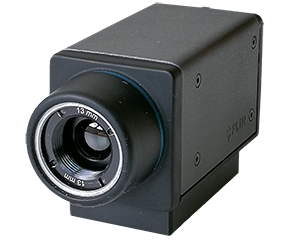
\includegraphics[width=5cm]{images/flir_a65_front.png} }}
      \qquad
      \subfloat{{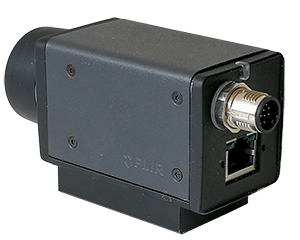
\includegraphics[width=5cm]{images/flir_a65_back.png} }}
      \caption{Termokamera FLIR A65}
      \label{fig:flir_a65}
  	\end{figure}

	\subsection{Softwarové nástroje}
    Pro získání dat z~termokamery je nutné vybrat vhodné SDK. Následně s~jeho pomocí vytvořit řídící aplikaci pro příjem dat a ovládání kamery. Ideální případ by nastal, pokud by bylo možné zvolit SDK s~rozhraním pro Javu a~integrovat jej do stejné aplikace jako navržený algoritmus.
    
    Pro algoritmus detekce bude vytvořená aplikace v~jazyce Java s~využitím knihovny OpenCV. Tato aplikace bude mít vytvořené grafické rozhraní pomocí platformy JavaFX \cite{javafx}. Grafické rozhraní ulehčí manipulaci s~daty a usnadní nastavení parametrů jednotlivých algoritmů.

Pro vyhodnocování a klasifikaci dat bude využit nástroj RapidMiner \cite{rapidminer}, který je v~tuto chvíli jeden z~nejvyužívanějších nástrojů pro data mining. Tento nástroj lze získat v~bezplatné community verzi, která má sice svá omezení, ale je pro potřeby této práce dostačující.
    
    \subsection{Volba SDK}
    Pro účely této práce by bylo nejvhodnější využít SDK ActiveGigE (\ref{section:sdk}). Poskytuje nejvíce funkcí již v~základu a je dostupné pro Javu, takže by jej bylo možné integrovat do aplikace s~detekčním algoritmem. Naneštěstí se jedná o~placené SDK a tak bylo nutné přejít k~alternativní volbě. 
    
    Jiné kompatibilní SDK, které by mělo rozhraní pro Javu neexistuje, takže bylo vybíráno na základě jednoduchosti a kvality dokumentace. Rozhodování probíhalo mezi JAI SDK a eBUS SDK, ale nakonec bylo rozhodnuto pro eBUS SDK, které je podstatně jednodušší a nabízí velké množství již implementovaných funkcionalit.
    
    \subsubsection{OpenCV}
    OpenCV \cite{opencv_library} je volně dostupná knihovna (pod licencí BSD), primárně určená pro zpracování obrazu. Je napsaná v~jazyce C/C++ a poskytuje rozhraní pro ostatní programovací jazyky jako je Java a Python. Všechny její operace jsou optimalizovány a navrhnuty pro zpracování dat v~reálném čase. Pro maximalizaci výkonu využívá hardwarové akcelerace a paralelní výpočty.
\chapter{Průzkum možných řešení}
Tato kapitola je zaměřena na hledání vhodného řešení zadaného problému. Vzhledem ke skutečnosti, že problém je dost specifický a nikdo jej ještě pomocí termokamery neřešil, jeho referenční řešení není známé. Jsou využity pouze znalosti získané při rešerši a je navrhnuto několik postupů, ze kterých bude vybrán ten nejvhodnější.

\section{Získávání dat z~kamery}
Před samotnou implementací algoritmů je nutné se zaměřit na získání dat. V~předchozí kapitole bylo popsáno, že se nejedná o~triviální úlohu a tak je potřeba vytvořit vlastní aplikaci pro nastavení a příjem dat z~kamery.

	\subsection{Aplikace pro přenos dat a komunikaci s~kamerou}
    V~rámci tvorby aplikace pro komunikaci s~kamerou, bylo nutné se seznámit s~poskytovaným rozhraním vybraného eBUS SDK. Dokumentace k~tomuto SDK je velmi detailní a tato část probíhala bez větších potíží. Bylo velmi snadné vytvoření jednoduché aplikace v~jazyce C++ pro připojení kamery, jejího nastavení a získání jednotlivých snímků. Problém nastal až při implementaci kontinuálního ukládání dat, kdy přes veškerou snahu se nedařilo tuto funkčnost zprovoznit. Aplikace se zasekávala, vracela chybová data a ukládání fungovalo nespolehlivě.
    
    Pro vypořádání se s~tímto problémem byla zvolena alternativa, a to využití aplikace eBUS Player z~ukázkových C++ kódů. Tato aplikace již obsahuje všechny nutné funkcionality pro správu připojení, nastavení a ukládání dat kamery. Bylo by možné pomocí této aplikace pouze data přenášet z~kamery, ukládat na disk a další práci nad daty provádět formou záznamu. Jako elegantnější řešení bylo rozšíření eBUS Playeru pro přenos dat do libovolného programovacího jazyka pomocí síťových soketů. Následné zpracování a třídění přenesených dat pak může probíhat pohodlněji ve vyšším programovacím jazyce. 
    
    V~této rozšířené aplikaci je možné nastavit všechna potřebná nastavení kamery pomocí uživatelského rozhraní a navázat komunikaci s~klientem. V~případě, že je komunikace navázána úspěšně, začnou se přijímaná data z~termokamery přenášet skrz soket. Při přenosu se nevyužije naplno propustnost síťového rozhraní, takže přenos není zahlcen a data klientem mohou být přijímány prakticky ihned. Obraz je tímto způsobem možné přenášet téměř v~reálném čase.
    
    Nutno podotknout, že součástí odesílaných souborů nejsou žádná metadata ani jiné hlavičky, které by popisovaly příchozí soubory. V~rámci práce to nebylo nutné, protože klientská aplikace vždy ví, jaká data má očekávat. 

	\subsection{Formát přenášených dat} \label{transmitted_data_format}    
    Aplikace pro příjímání dat z~kamery umožňuje ukládat data buď v~komprimovaných formátech jako je JPG a BMP, nebo v~nekomprimovaných jako je TIFF a nebo v~surovém formátu, kde jsou obsahem jednotlivé hodnoty z~detektoru. Vzhledem k~tomu, že je vždy lepší pracovat s~co nejméně komprimovanými daty, je rozhodnuto pro přenos surových dat. Tato nezpracovaná data je z~termokamery možné přijímat ve dvou různých formátech. To se řídí dle nastaveného režimu v~protokolu GenICam.
       
    \begin{description}[align=left]\label{description:transfer_data_modes}
      \item [Signal linear mode] V~tomto režimu odpovídají jednotlivé pixely obrazu hodnotám signálu z~maticového detektoru. Tento signál toho sám o~sobě nic moc neříká, může být pouze převeden na teplotu. Pro převod signálu S~na teplotu T v~kelvinech slouží vzorec:

      \begin{equation}
      	T_{[K]}=\frac{B}{\ln{\left(\frac{R}{S - O} + F\right)}},
      \end{equation}

      kde hodnoty R, B, F, O~jsou uloženy v~registrech kamery a lze je zjistit v~uživatelském rozhraní přehrávače eBUS a nebo dotazem do GenICam protokolu.

      \item [Temperature linear mode]\label{item:temperature_linear} Data získaná v~tomto režimu při vynásobení konstantou $K$ přímo odpovídají teplotám. Hodnota konstanty $K$ se liší dle typu kamery a také dle rozlišení signálu nastaveného v~protokolu GenICam. Pro kameru A65 teplotu $T$ v~kelvinech lze ze signálu $S$ získat jako:
      \begin{equation}
		T_{[K]}=0.04 \times
S~\end{equation} 
      
      pro vysoké rozlišení signálu a 
      
      \begin{equation}
		T_{[K]}=0.4 \times
S~\end{equation}
       
       pro nízké rozlišení signálu.
    \end{description}
    
    Z~výše uvedených způsobů získání teplot ze surových dat je zřejmé, že využití režimu Temperature linear je výpočetně jednodušší a pohodlnější, protože není potřeba dotazovat protokol a používat výpočetně náročný vzorec s~dělením a logaritmem pro každý pixel obrazu.   
    Přenášená data jsou tedy vždy odesílána neupravena, v~14-bitové kvalitě a ve formátu Temperature linear s~vysokým rozlišením.
    
	\subsection{Oblast snímání}
  	Nemělo by smysl snímat celé obrazové pole, protože se v~něm vyskytuje regál i osoba. V~tomto případě je zajímavé se zaměřit pouze na oblast, kde se může vyskytovat ruka. To znamená, snímat pouze bezprostřední oblast před regálem.

      Velikost této oblasti byla experimentálními způsoby stanovena pro obě kamery na hodnotu 640 $\times$ 150 pixelů. Oblast je záměrně o~něco širší než by bylo potřeba. Je to z~toho důvodu, že během snímání může kdykoliv nastat kalibrace NUC a přerušit tím snímání. Tím, že bude oblast o~něco větší, bude získáváno více snímků ruky a tím snížena pravděpodobnost, že NUC překazí snímání v~důležitý moment. 
      
      V~případě, že by kamera (13 mm) měla rychlejší snímkovací frekvenci, byla by pro ni oblast s~výškou 70 pixelů dostačující. Příklad výřezu oblasti a jeho neupraveného zdroje je zobrazen na obrázku \ref{fig:camera_2_sample_image_small} a \ref{fig:camera_2_sample_image_full}.
    
    \begin{figure}[h]
      \centering
      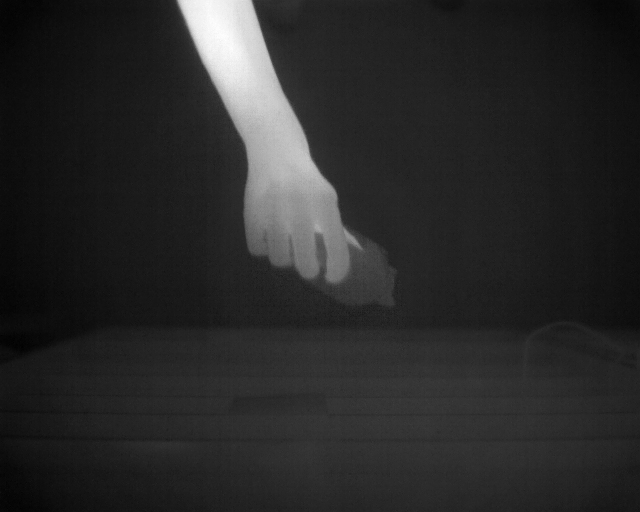
\includegraphics[width=0.8\textwidth]{images/camera_2_sample_image_full.jpg}
      \caption{Neupravený snímek v~plné velikost}
      \label{fig:camera_2_sample_image_full}
    \end{figure}  

    \begin{figure}[h]
      \centering
      
\includegraphics[width=0.8\textwidth]{images/camera_2_sample_image_small.jpg}
      \caption{Výřez oblasti zájmu neupraveného snímku}
      \label{fig:camera_2_sample_image_small}
    \end{figure}  

	\subsection{Redukce oblasti}\label{section:area_reduction}
    Kamera A65 v~sobě mimo jiné nese registry pro možnost snímání pouze výřezu obrazového pole. Díky tomu je možné z~kamery rovnou přijímat redukovanou oblast. Tyto registry se nastavují v~protokolu GenICam a je možné je změnit v~uživatelském rozhraní upraveného eBUS Playeru. Registry pro výběr oblasti jsou označeny jako: Width, Height, OffsetX, OffsetY. Jejich hodnoty pro jednotlivé kamery použité v~práci jsou uvedeny v~tabulce \ref{table:region_of_interest_settings}. Posun v~ose Y je nastaven tak, aby se zaznamenávaná ruka na snímku vyskytovala přibližně uprostřed.

    \begin{table}[h]
      \centering
      \begin{tabular}{|c|c|c|}
        \hline
        \rowcolor{Blue}
        \color{White}\textbf{Parametr} & \color{White}\textbf{Kamera 1 (13 mm)} & \color{White}\textbf{Kamera 2 (25 mm)}\\ \hline
        šířka & \multicolumn{2}{|c|}{640 pixelů}   \\ \hline
        výška & \multicolumn{2}{|c|}{150 pixelů}   \\ \hline
        posun v~ose X & \multicolumn{2}{|c|}{ 0 pixelů} \\ \hline
        posun v~ose Y & 190 pixelů & 170 pixelů \\ \hline
      \end{tabular}
      \caption{Hodnoty registrů pro výběr oblasti zájmu}
      \label{table:region_of_interest_settings}
    \end{table}
    
    Vyhotovení výřezu obrazového pole rovnou na straně termokamery je výhodné v~tom, že je přenos oproštěn od nezajímavých dat a není zbytečně zatěžováno síťové rozhraní. Pokud by se přeci jen přenášel celý snímek, musela by určitá redukce obrazového pole stejně proběhnout na straně klientské aplikace, protože většina algoritmů má velkou výpočetní náročnost a není nutné je provádět nad obrazem v~plném rozlišení.

  	\subsection{Proces snímání}
 	Snímání probíhalo v~Laboratoři zpracování obrazu na FIT ČVUT v~Praze. Teplota se v~této místnosti pohybovala v~rozmezí běžné pokojové teploty a to mezi 19 - 24 \textdegree{}C. Teplota zboží v~regále a podlahy v~podobných relacích. 
 
	Regál je vysoký 200 cm a široký 80 cm. Vzdálenost umístění kamer od země je uvedena na obrázku \ref{fig:shelf_scheme}. Reálné umístění kamery a podoba regálu je vidět na fotografii \ref{fig:shelf_setup}. Kamera je umístěna v~souladu s~posunem uvedeným v~\ref{section:area_reduction}, aby se ruka sahající do regálu vyskytovala přibližně uprostřed, kde obraz dosahuje nejvyšší kvality. Optika kamery je manuálně zaostřena přibližně do 3/4 regálu vzdálenosti od podlahy. 

  \begin{figure}[h]
    \centering
    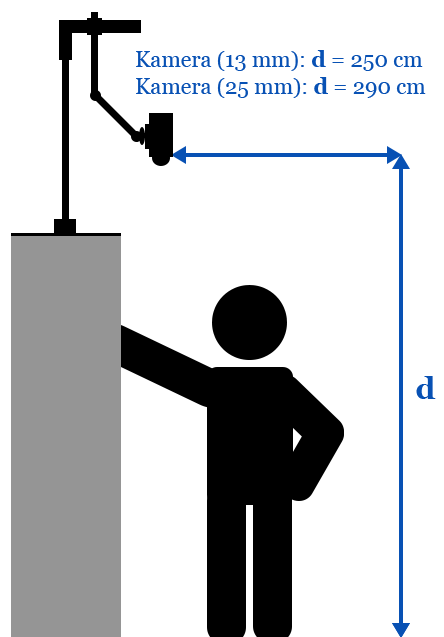
\includegraphics[width=0.5\textwidth]{images/camera_setup_scheme.png}
    \caption{Schéma umístění kamery}
    \label{fig:shelf_scheme}
  \end{figure}  

  \begin{figure}[h]
    \centering
    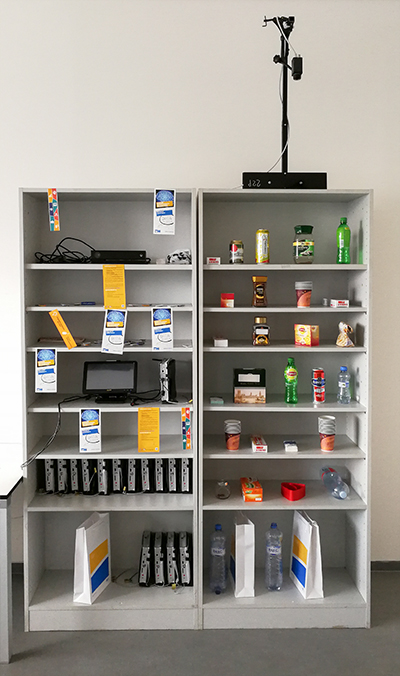
\includegraphics[width=0.6\textwidth]{images/shelf_setup.jpg}
    \caption{Fotografie umístění kamery}
    \label{fig:shelf_setup}
  \end{figure}    

\section{Předzpracování dat}
Ještě před začátkem aplikace algoritmů je data nutné převést z~binární podoby na teploty. Tyto teploty normalizovat do nového rozsahu, aby je bylo možné zobrazit. Poté už je možné pracovat se snímkem, který je nutno obrazově předzpracovat. 

Zpracování snímku probíhá v~následujícím pořadí: převod binárních dat, normalizace teplot, expoziční úpravy, odstranění šumu. Efekt těchto kroků je zobrazen na obrázku \ref{fig:camera_2_image_preprocessing}. 

\begin{figure}[h]
  \centering
  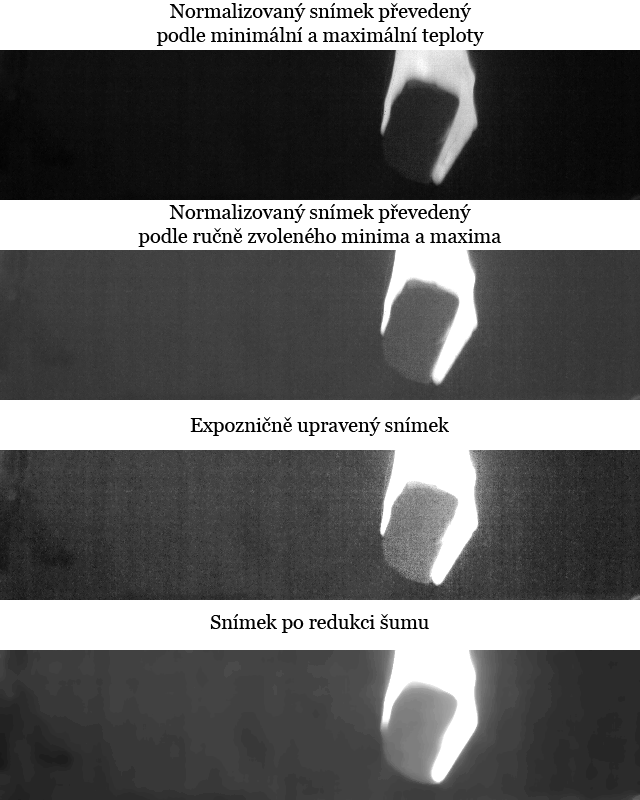
\includegraphics[width=0.8\textwidth]{images/camera_2_image_preprocessing.png}
  \caption{Jednotlivé kroky předzpracování snímku}
  \label{fig:camera_2_image_preprocessing}
\end{figure} 

	\subsection{Převod binárních dat a normalizace teplot}
    Binární data z~kamery jsou snímána v~Temperature linear režimu, takže je možné je snadno převést podle \ref{item:temperature_linear} na teplotu v~kelvinech. Teplotu v~kelvinech je ještě vhodné převést na běžnější teplotu v~\textdegree{}C a to pomocí jednoduchého vzorce:
    
    \begin{equation}
 	   T_{[C]}= T_{[K]} - 273.15,  
    \end{equation}
    
	kde $T_{[C]}$ je nová teplota v~\textdegree{}C a $T_{[K]}$ teplota v~K.
    
    Tyto teplotní data je nutné normalizovat do nového rozsahu, aby bylo možné je rozumně zobrazit. Nejjednodušším způsobem je ve snímku vyhledat minimální a maximální teplotu a všechny teploty normalizovat pomocí vzorce:
    
    \begin{equation}
  	  x_{norm} = \frac{(newMax - newMin) }{ (oldMax - oldMin)}* (x - oldMax) +newMax,
    \end{equation}
    
    kde $x$ je hodnota před normalizací, $x_{norm}$ je nová hodnota, $oldMax$ a $oldMin$ jsou nalezené minimální a maximální teploty v~snímku a $newMax$ a $newMin$ je nový rozsah hodnot. Většina algoritmů z~knihovny OpenCV pracuje pouze s~8-bitovými maticemi, takže je vhodné data převádět rovnou do 8-bitové podoby. Z~toho plyne, že hodnota $newMax$ je vždy 255 a $newMin$ vždy 0.
    
    Způsob normalizace snímku pomocí nalezené minimální a maximální teploty se ukázal jako nevhodný, protože zboží bylo stěží rozeznatelné i pro člověka. Hledání hodnot $oldMax$ a $oldMin$ tedy není automatizováno a jejich volba probíhá ručně.
   	
    \subsection{Úprava expozice a odstranění šumu}
    Normalizovaný snímek je pro zvýraznění teplotních rozdílů expozičně upraven. Proběhne zvýšení kontrastu a následné snížení jasu. Tímto procesem se na snímku vygeneruje velké množství šumu, které je potřeba zredukovat.
    
    Šum je odstraněn nejprve pomocí mediánového filtru \cite{huang1979fast} a následně ještě pomocí bilaterálního filtru \cite{tomasi1998bilateral}, který zachovává hrany.
    
\section{Řešení segmentací na základě teplot objektů} 
Prvním navrženým řešením je segmentace obrazu pouze na základě teplot. Toto řešení se dá považovat za velmi naivní, ale nemusí být hned jasné, v~čem spočívá problém.

Ještě před zpracováním snímku je možné z~jednotlivých pixelů získat konkrétní teploty. V~oblasti zájmu se může objevit pouze ruka, zboží a podlaha. Pro zamýšlení se nad dalším postupem je nutné zjistit rozmezí teplot těchto tří objektů.

Teplotně se ruka pohybuje přibližně od 26 \textdegree{}C a není zde moc co vymýšlet. Problém nastává s~určením rozsahu teploty zboží. Zboží se totiž v~průběhu manipulace zahřívá od ruky a nebo naopak ochlazuje okolním vzduchem. Pokud se teplota v~místnosti změní, některé zboží na tuto změnu reaguje rychleji a některé pomaleji v~závislosti na tepelné vodivosti. Zboží má oproti podlaze teplotu průměrně o~0.2 - 0.5 \textdegree{}C vyšší, ale může se stát, že některé zboží bude mít v~některých chvílích i nižší teplotu než má podlaha (díky tepelné vodivosti a změně teploty vzduchu). 

Dalším faktorem je nestabilita výstupu z~termokamery. Mezi jednotlivými korekcemi NUC (\ref{section:nuc}) se teplota s~postupem času nelineárně mění. Tento posun může být v~některých situacích až 1 \textdegree{}C za minutu. 

Najít přesný teplotní rozsah pro zboží není možné a tato úloha se tímto způsobem řešit nedá.

\clearpage

\section{Řešení s~využitím hranové detekce}\label{section:edge_detection_solution}
Druhým navrženým řešením je využít hranovou detekci pro získání hran objektu a prahování pro získání ruky. Prvním krokem je získání masky ruky z~předzpracovaného snímku. Masku je možné získat více způsoby. Byly experimentálně vyzkoušeny tyto postupy: binární prahování, Otsu prahování, adaptivní prahování, segmentace pomocí hranové detekce. Ukázalo se, že čím složitější metoda byla využita, tím byly výsledky horší, protože tyto adaptivní algoritmy se pro povahu úlohy nehodí. 

Pokud předzpracovaný snímek obsahuje ruku, tak si lze na obrázku \ref{fig:camera_2_image_preprocessing} všimnout, že pixely ruky jsou velmi jasné. Začínají průměrně od hodnoty 180 (v~rozmezí 0 černá a 255 bílá) a je snadné je rozlišit od tmavého pozadí. Pro získání masky ruky je  využito jednoduché, ale velmi rychlé, binární prahování s~hodnotou prahu 180.

Na snímku je dále patrné, že kolem ruky vzniká záře, která nenese žádnou informaci a lze ji považovat za šum. Tento šum se dá velmi obtížně redukovat, protože vzniká kolem celé oblasti ruky a ovlivňuje i zboží. Alespoň pro částečné odstranění této záře je využito morfologické operace dilatace \cite{serra1982image} s~obdélníkovým jádrem. Je však nutné počítat s~tím, že dilatace zmenšuje oblast pro zboží.

Aby byly hledány pouze relevantní hrany, je na snímku vyhledána oblast zájmu a ohraničena pomocí ohraničujícího obdélníku (bounding boxu). Oblast zájmu je nalezena pomocí vyhledání největší kontury. Pomocí největší kontury se pak řídí šířka oblasti, která je ještě vhodně zvětšena. Výška oblasti je vždy celá velikost snímku, protože zboží dost často přesahuje právě před rukou. Pokud není tato oblast nalezena, ruka se na snímku nevyskytuje a nemá smysl dále vyhodnocovat.

V~případě, že je nalezena oblast zájmu, je dalším krokem vyhledání hran. Stejně jako u~způsobu segmentace ruky bylo pro detekci hran experimentálně vyzkoušeno několik detektorů (Prewittův, Sobelův, Sacharrův, Laplaceův, Cannyho) s~různými způsoby nastavení a předzpracování obrazu. Ve všech případech poskytoval Cannyho hranový detektor \cite{canny1986computational} nejpřesnější výsledky. V~případech velmi malé jasové změny (teplota zboží blízko teplotě podlahy), nacházel též Cannyho detektor nejrelevantnější hrany.

Na nalezené hrany je dále v~několika iteracích aplikována dilatace a eroze pro spojení blízkých hran a odstranění hran malých, které jsou pravděpodobně šum. 

Výsledný snímek hran zboží vznikne jako binární součet snímku hran a~inverze binární masky ruky. Na tomto snímku se pak vypočtou předem dané atributy kontur (uvedeny v~následující kapitole \ref{section:attributes}), podle kterých je možné ho klasifikovat. Algoritmus je též graficky znázorněn ve vývojovém diagramu \ref{fig:edge_detection_diagram}.

\begin{figure}[h]
  \centering
  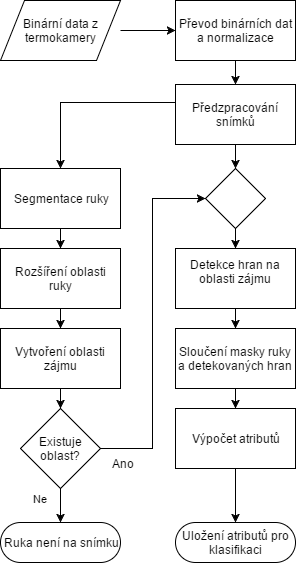
\includegraphics[width=0.6\textwidth]{images/edge_detection_diagram.png}
  \caption{Vývojový diagram algoritmu s~využitím hranové detekce}
  \label{fig:edge_detection_diagram}
\end{figure} 

    \subsection{Problémy}
    Toto řešení se mimo jiné ukázalo jako velmi citlivé na pohyb ruky. V~případě, že se ruka pohybuje rychle, na snímku se projeví pohybová neostrost, která díky nižší jasové hodnotě než má ruka, není segmentována. Následně se po aplikaci Cannyho detektoru jeví artefakty pohybové neostrosti ruky jako hrany zboží a tyto snímky jsou chybně klasifikovány. Problém s~nadbytečnými hranami způsobuje i záře, která se vyskytuje kolem ruky.

	\subsection{Vyhodnocení}
    Výsledky tohoto řešení se pohybovali v~rozmezí 65 - 75 \% celkové přesnosti klasifikace v~závislosti na použitém klasifikátoru. Detailnější informace nejsou dále diskutovány, protože toto řešení nebylo shledáno jako konečné a bylo navrženo lepší, které je následně detailněji vyhodnoceno.
         
\clearpage

\section{Řešení pomocí dynamického odčítání pozadí} \label{section:background_substract_solution}
Toto řešení bylo s~využitím nových znalostí a postřehů navrženo pro zlepšení předchozích výsledků. %Obsahuje více kroků, než předchozí řešení a jednotlivým metodám jsou parametry nastaveny experimentálně %Řešení využívá více různých po sobě jdoucích operací, které byly experimentálně nastaveny parametry, které byly nalezeny a shledány jako nejlepší kombinací.

V~paměti je uchováváno průběžně aktualizující se pozadí. Je to z~důvodu, že obraz z~termokamery není plně stabilní a mezi jednotlivými snímky se v~čase mění. Největší změna v~obraze se vždy projeví po  kalibraci NUC a je na ni nutné co nejrychleji reagovat. Z~toho důvodu nebylo použité pouze průměrování pozadí, ale je využito akumulovaní pozadí s~předem danou váhou. Při akumulovaní pozadí jsou jednotlivé pixely nového pozadí vypočteny jako:

\begin{equation}
	acc(x, y) = (1 - \alpha) \times acc(x, y) + a \times src(x,y),
\end{equation}

kde src(x, y) je hodnota vstupního pixelu na souřadnicích (x, y), acc(x, y) je hodnota pixelu akumulovaného pozadí v~paměti a $\alpha$ je váha nového pixelu. Čím větší je $\alpha$, tím je schopné se pozadí rychleji adaptovat na změnu prostředí. Pro $\alpha$ byly testovány hodnoty od 0,1 až do 0,5 a nakonec se pro tento typ úlohy ukázala jako nejlepší hodnota 0,3.

Od aktuálního snímku je odečteno pomocí \cite{opencvMOG} průběžně aktualizující se pozadí a z~této operace vznikne maska popředí. Tato maska je použita k~získání reálného popředí. Na získané popředí je stejně jako v~řešení \ref{section:edge_detection_solution} aplikováno binární prahování pro zisk masky ruky a tato maska je dilatací rozšířena. V~případě, že žádná maska ruky neexistuje, je snímek použit pro výpočet nového pozadí. Efekty těchto kroků je možné vidět na obrázku \ref{fig:camera_2_mog_preprocessed_substracted_hand}.

\begin{figure}[h]
  \centering
  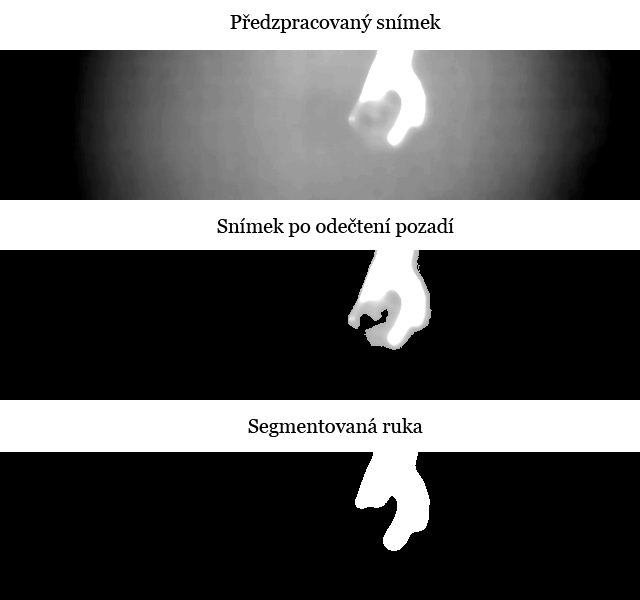
\includegraphics[width=0.8\textwidth]{images/camera_2_mog_preprocessed_substracted_hand.png}
  \caption{Ilustrace operací získání popředí snímků a segmentace ruky}
  \label{fig:camera_2_mog_preprocessed_substracted_hand}
\end{figure} 

Maska ruky je invertována a použita pro maskování popředí. Tímto způsobem na snímku zůstane šum a možné zboží, které je nutné nějakým způsobem zpracovat. Prvním aplikovaným způsobem je odstranění možného zboží od šumu ve formě záře kolem ruky. Tento postup spočívá v~nalezení kontur, jejich aproximaci pomocí algoritmu Douglas-Peucker \cite{opencvaproxpoly}, nalezení konvexní obálky a vyhledání konvexních defektů. Mezi konvexními defekty je nalezen ten s~největší hloubkou, který se pravděpodobně nachází v~oblasti mezi palcem a ostatními prsty. Jednotlivými body defektů jsou protnuty úsečky černé barvy a vhodné velikosti, které v~některých případech zajistí oddělení šumu od zboží. Tento postup je ilustrován na obrázku \ref{fig:camera_2_mog_goods_processing}.

\begin{figure}[h]
  \centering
  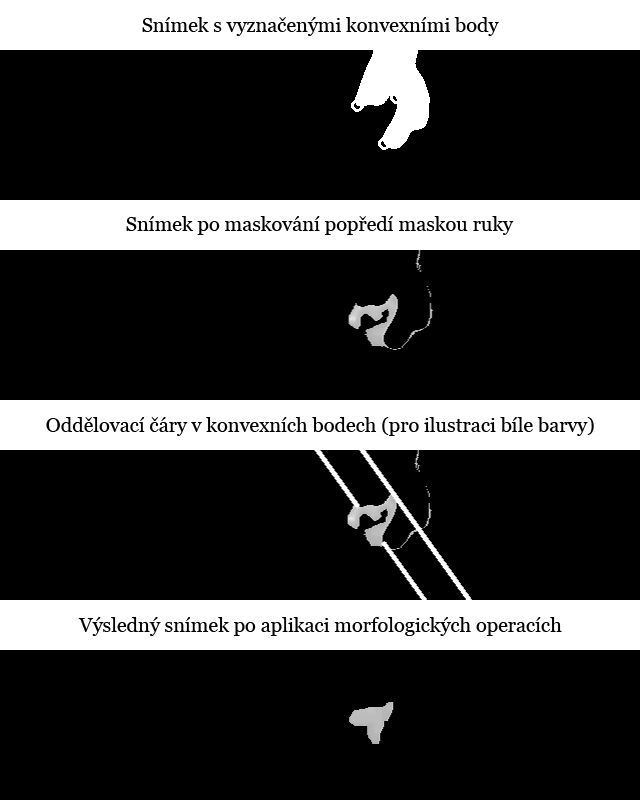
\includegraphics[width=0.8\textwidth]{images/camera_2_mog_goods_processing.png}
  \caption{Proces zpracování snímku zboží}
  \label{fig:camera_2_mog_goods_processing}
\end{figure} 

Na oddělené fragmenty obrazu jsou dále v~několika krocích vhodně aplikovány morfologické operace a to eroze a poté dilatace. Tento snímek může být zbylé zboží nebo šum a jsou na něm vypočteny předem dané atributy pro klasifikaci. Algoritmus je taktéž popsán ve vývojovém diagramu \ref{fig:edge_detection_diagram}. 

\begin{figure}[h]
  \centering
  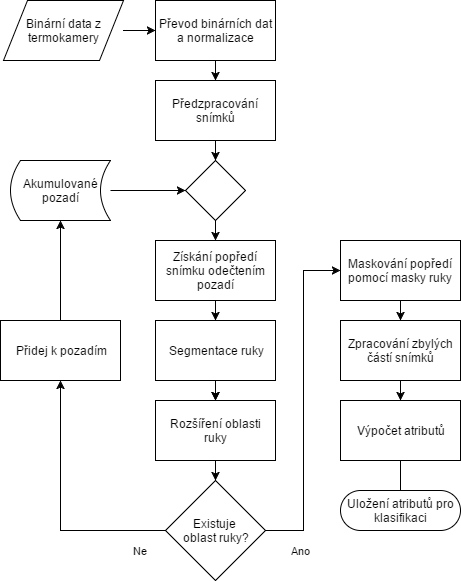
\includegraphics[width=0.8\textwidth]{images/mog_detection_diagram.png}
  \caption{Vývojový diagram algoritmu dynamického odečítání pozadí}
  \label{fig:mog_detection_diagram}
\end{figure} 

	\subsection{Úskalí řešení} \label{section:background_substract_problems}
    Největší nevýhodou tohoto řešení je, že je silně závislé na uloženém pozadí v~paměti. V~případě, že proběhne NUC kalibrace a do paměti se nestačí načíst dostatečný počet snímků nového pozadí, proběhne operace odečtení pozadí chybně. V~tomto případě jsou pak vypočteny nesmyslné hodnoty atributů, protože se jako zboží  tváří skoro celá oblast snímku. Pro ilustraci je tento případ zobrazen v~obrázku \ref{fig:camera_2_apply_mog_after_nuc}.
    
    Dalším problémem je, stejně jako v~algoritmu \ref{section:edge_detection_solution}, rychlý pohyb ruky při kterém se projevuje pohybová neostrost, která rozšiřuje pomyslnou oblast zboží.
    
    \begin{figure}[h]
      \centering
      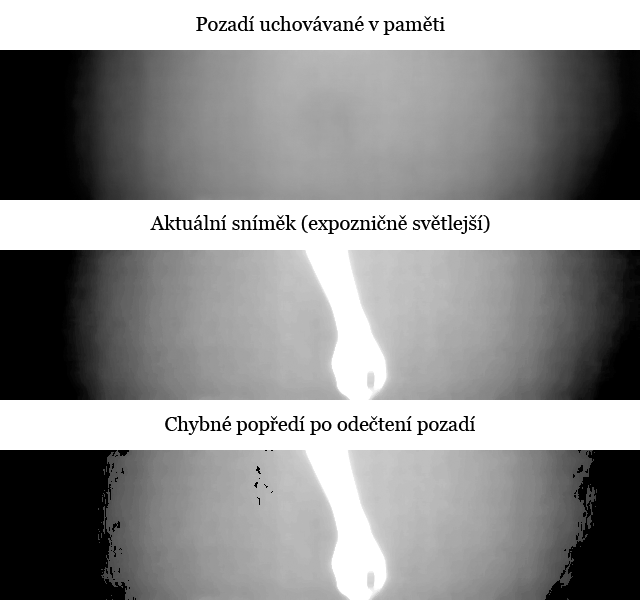
\includegraphics[width=0.8\textwidth]{images/camera_2_apply_mog_after_nuc.png}
      \caption{Chybně získané popředí kvůli změně expozice aktuálního snímku}
      \label{fig:camera_2_apply_mog_after_nuc}
	\end{figure} 

	\subsection{Vyhodnocení}
    Toto řešení bylo vybráno jako finální a jeho vyhodnocení je možné detailněji nalézt v~následující kapitole \ref{chapter:choosen_solution}.
    
\clearpage

\section{Řešení s~kombinací RGB obrazu}\label{section:combining_rgb_and_thermal}
U~všech řešení pouze s~termokamerou je největším problémem rozlišit pozadí (podlahu) od zboží kvůli velmi podobným teplotám a záři, která vzniká kolem ruky. V~případě, že by bylo možné striktně oddělit pozadí od popředí (ruka se zbožím), celý problém by se značně zjednodušil, protože segmentovat zboží od ruky lze díky rozdílným teplotám velmi snadno. 

V~tomto ohledu by bylo lepší využít klasickou kameru s~viditelným spektrem pro získání masky popředí. Tuto masku pak aplikovat na termovizní snímek a následně na něm segmentovat ruku a detekovat zboží. Tento snímek pak ještě vhodně zpracovat a vypočítat na něm atributy ke klasifikaci.

Pro otestování tohoto řešení byla využita externí RGB webkamera a ukázalo se, že toto řešení přináší dva velmi podstatné problémy.

    \subsection{Synchronizace kamer}
    Prvním problémem je sladění snímků z~různých kamer. Kamery spolu nejsou nijak propojeny a tak procesorové hodiny tikají na každé kameře jinak. Pořizované snímky v~čase jsou rozdílné a je možné nalézt snímky, které při pohybu ruky neodpovídají žádným snímkům z~druhé kamery. Jednoduše řečeno, kamery nemají synchronizované snímání a tak je u~každé kamery snímek vyhotoven v~jiný čas. Navíc u~toho u~termokamery vstupuje kalibrace NUC, při které kamera žádné snímky nepřenáší a občas se objevují i chyby přenosu, kdy požadovaný snímek nemusí být vůbec obdržen. 

    Snímky nelze přesně synchronizovat již po přijmutí z~kamer, protože by tímto způsobem vznikalo mnohem více chyb a výsledný algoritmus by byl méně přesný než v~případě jedné kamery.

    Synchronizaci snímků je možné řešit pouze hardwarově. Některé průmyslové kamery bývají vybaveny konektory, které slouží právě k~synchronizaci více kamer. Je možné propojit několik kamer, kdy synchronizace snímání probíhá vůči jedné vybrané kameře (master, slave režim). Synchronizaci je možné konfigurovat pomocí protokolu GenICam. Termokamera dostupná v~práci má k~dispozici synchronizační konektor, ale nebyla k~dispozici druhá kamera, která by s~ní byla kompatibilní.

	\subsection{Perspektiva snímků}
    Druhým problémem je rozdílná perspektiva snímků. Různé kamery nikdy nebudou mít stejnou optickou soustavu. Tento fakt je způsoben různými optickým vadami objektivů a často se objektivy liší i v~ohniskové vzdálenosti. Tyto skutečnosti pak ovlivňují výsledné zarovnání snímků. Na obrázku \ref{fig:webcam_sample} lze nejdříve vidět rozměrově neupravený snímek z~webkamery, který je následně oříznutý na oblast termokamery \ref{fig:visible_cropped_to_thermal}. V~posledním obrázku \ref{fig:visible_thermal_combined} jsou oba snímky prolnuty a lze snadno pozorovat, že i přes stejnou scénu na sebe snímky, právě díky rozdílné perspektivě, nelze přesně zarovnat.

    \begin{figure}[h]
      \centering
      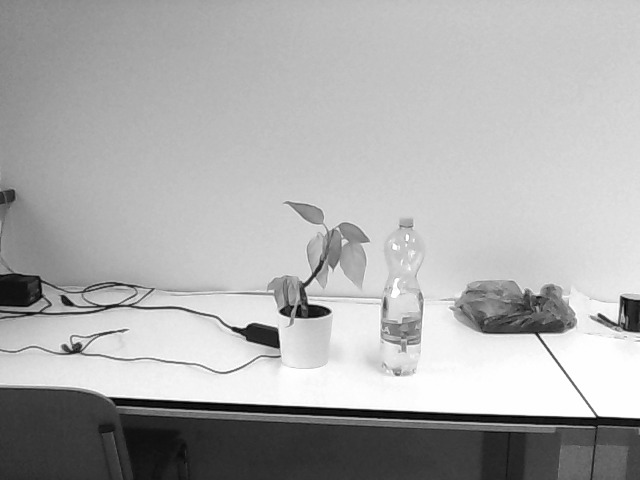
\includegraphics[width=0.6\textwidth]{images/webcam_sample.png}
      \caption{Ukázkový snímek snímaného obrazového pole webkamery}
      \label{fig:webcam_sample}
    \end{figure} 

    \begin{figure}[h]
      \centering
      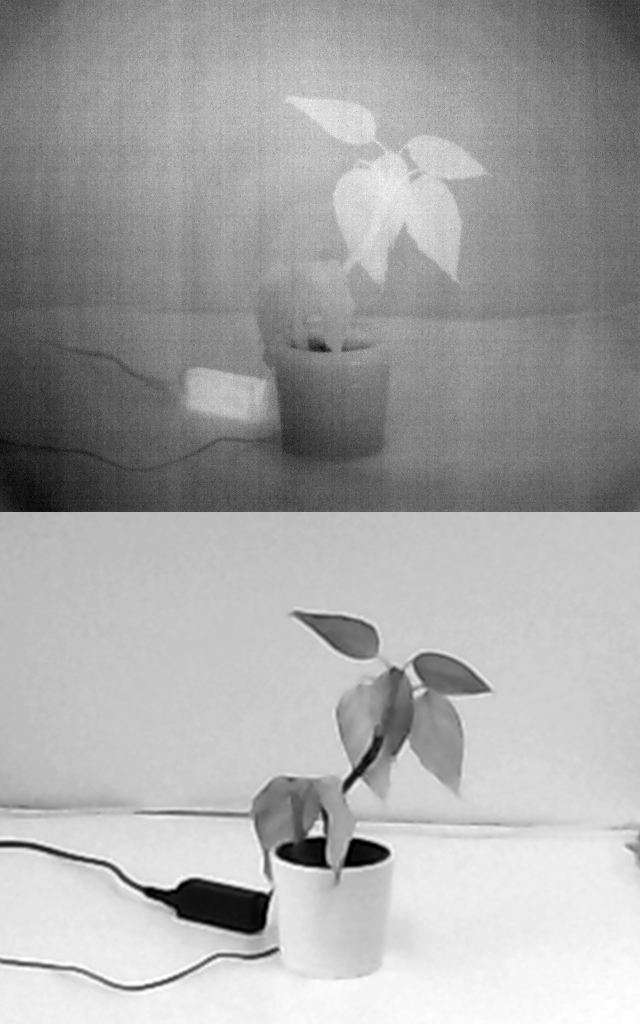
\includegraphics[width=0.6\textwidth]{images/visible_cropped_to_thermal.png}
      \caption{Snímek z~webkamery oříznutý k~obrazovému poli termokamery}
      \label{fig:visible_cropped_to_thermal}
    \end{figure} 

    \begin{figure}[h]
      \centering
      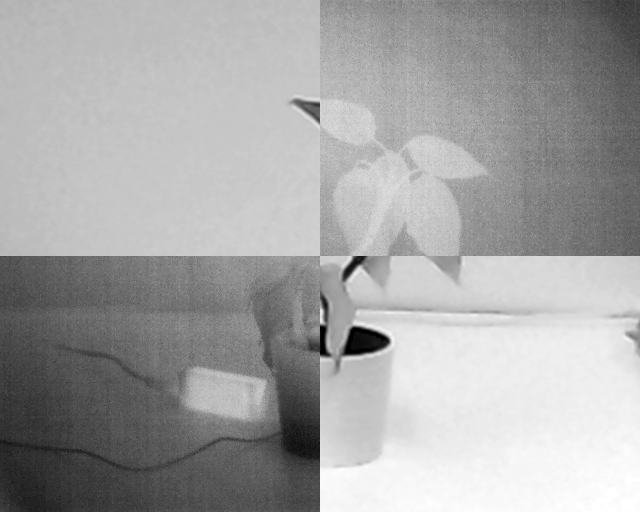
\includegraphics[width=0.9\textwidth]{images/visible_thermal_combined.png}
      \caption{Ručně sloučené snímky z~webkamery a termokamery}
      \label{fig:visible_thermal_combined}
    \end{figure} 

    Řešením je nalezení transformační matice homografie pro mapování obrazu webkamery na plochu obrazu termokamery. V~problému detekce zboží v~ruce to znamená hledání několika transformačních matic, protože perspektiva se mění v~závislosti na vzdálenosti snímaného objektu a ruka na snímku se může objevit v~několika rovinách. Čím více je nalezeno transformačních matic pro různé vzdálenosti, tím jsou výsledky mapování přesnější. V~knihovně OpenCV je hledání transformační matice homografie již implementováno metodou findHomography z~balíku calib3d.

	\subsection{Shrnutí}
    Toto řešení nakonec nebylo implementováno hlavně kvůli problémům se synchronizací kamer, které v~rámci práce nebylo možné vyřešit. Pro případné navázaní na tuto práci je alespoň uveden vývojový  diagram \ref{fig:visible_thermal_detection_diagram} algoritmu.

    \begin{figure}[h]
      \centering
      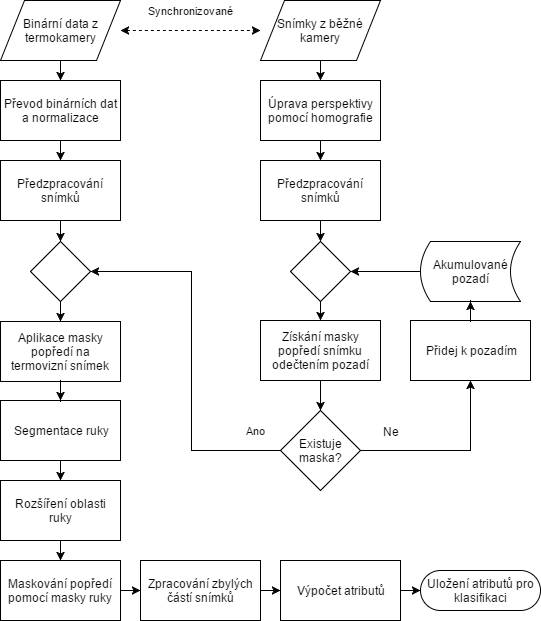
\includegraphics[width=0.9\textwidth]{images/visible_thermal_detection_diagram.png}
      \caption{Vývojový diagram algoritmu využívající kombinace běžného a termografického snímku}
      \label{fig:visible_thermal_detection_diagram}
    \end{figure} 


    




\chapter{Zvolené řešení a jeho vyhodnocení}\label{chapter:choosen_solution}
Finálním vybraným řešením pro vyhodnocení je řešení s~termokamerou a algoritmem dynamického odčítání pozadí. Detaily algoritmu jsou uvedeny v~\ref{section:background_substract_solution} a zde je uvedeno pouze jeho stručné shrnutí. 

\section{Shrnutí řešení}
V~paměti je průběžně aktualizováno pozadí vůči kterému se vyhodnocuje právě načtený snímek. V~případě, že je snímek detekován jako pozadí, aktualizuje se s~jeho pomocí to v~paměti. V~opačném případě je získané popředí snímku, na kterém se dále segmentuje ruka. Pomocí invertované masky ruky je získáno popředí bez ruky, na kterém proběhne redukce artefaktů ve formě šumu a jako poslední krok je výpočet atributů pro klasifikaci.

\section{Volba atributů}\label{section:attributes}
Pro řešení bylo zvoleno celkem 20 atributů zaměřující se na vlastnosti kontur. Atributy související s~jasem, histogramem a podobnými vlastnostmi obrazu nebyly použity, protože výstup z~kamery se v~čase mění a není možné zajistit jeho stabilitu.

Zvolené atributy jsou rozděleny do dvou skupin. Na atributy týkající se vlastností největší nalezené kontury a souhrnné atributy všech nalezených kontur. Atributy vypočítávány na největší nalezené kontuře jsou:
\begin{description}
\item [Délka kontury (Perimeter)]
\item [Plocha kontury (Area)]
\item [Minimální průměr vepsané kružnice (Minimum diameter)]
\item [Maximální průměr vepsané kružnice (Maximum diameter)]
\item [Délka konvexní obálky (Convex perimeter)]
\item [Plocha konvexní obálky (Convex area)]
\item [Formfaktor (Formfactor)] získán jako 
    \begin{equation}
        \frac{4 \times \pi \times Area}{Perimeter^{2}}        
    \end{equation}
\item [Kulatost (Roundness)] získána jako 
    \begin{equation}
        \frac{4 \times Area}{\pi \times \text{Maximum diameter}^{2}}
    \end{equation}
\item [Poměr stran (Aspect ratio)] získán jako
	\begin{equation}
        \frac{\text{Maximum diameter}}{\text{Minimum diameter}}
	\end{equation}
\item [Konvexita (Convexity)] získána jako
	\begin{equation}
        \frac{\text{Convex perimeter}}{Perimeter}
	\end{equation}
\item [Pevnost (Solidity)] získána jako
	\begin{equation}
        \frac{Area}{\text{Convex area}}
	\end{equation}
\item [Kompaktnost (Compactness)] získána jako
	\begin{equation}
        \frac{\sqrt{\frac{4}{\pi} \times Area}}{\text{Maximum diameter}}
	\end{equation}
\item [Rozsah (Extent)] získán jako
	\begin{equation}
        \frac{Area}{\text{Maximum diameter} \times \text{Minimum diameter}} .
	\end{equation}
\end{description}
Atributy vypočítávané na všech nalezených konturách jsou:

\begin{description}
\item [Počet kontur]
\item [Součet ploch kontur]
\item [Minimální plocha kontury]
\item [Průměrná plocha kontury]
\item [Součet délek kontur]
\item [Minimální délka kontury]
\item [Průměrná délka kontury.]
\end{description}


\section{Rozdělení snímků do tříd}
Před klasifikaci, je nejdříve nutné snímky rozdělit do několika skupin. Klasifikačními skupinami jsou prázdná ruka a ruka se zbožím, ale pro správnou funkčnost uvedeného algoritmu je ještě nutné v~paměti uchovávat pozadí. Čím více snímků pozadí bude při vyhodnocování k~dispozici, tím budou výsledky přesnější.

Snímky jsou uchovávány jako binární soubory obsahující data v~podobě signálů, takže je nutno vytvořit speciální aplikaci pro jejich zobrazení a následné rozřazení do tříd. Pomocí této aplikace bylo ručně anotováno celkem 910 snímků prázdné ruky a 973 snímků ruky se zbožím. Všechna anotovaná pozadí byla získána pomocí aplikace s~algoritmy a ručně zkontrolovány pomocí aplikace pro anotování. Těchto pozadí je celkem 2173.

Navzdory tomu, že byly při práci využity dvě kamery, budou klasifikovány snímky pouze z~kamery (13 mm). Je to z~toho důvodu, že v~nasnímaných datasetech kamery (25 mm) se vyskytuje množství chyb, které vznikaly nevypočitatelně, kvůli její technické závadě. 

Celkem se tedy bude vyhodnocovat 1244 anotovaných snímků z~kamery (13 mm), z~toho 741 snímků ruky a 503 snímků ruky se zbožím, s~pomocí 2031 snímků pozadí.


\section{Klasifikace}
Před samotnou klasifikací jsou ještě jednotlivé hodnoty atributů normalizovány. Následně je spouštěna detekce anomálií a z~datasetu jsou některé záznamy odstraněny. Odstraněni probíhá pokud se součet délek kontur přibližuje celkové možné ploše obrazového pole. Tyto záznamy jsou očividně chybné a vznikají nejčastěji ihned po NUC, kdy ještě není dostatečně aklimatizováno uložené pozadí a při operaci odčítání pozadí se celý snímek bere jako popředí (ilustrováno v~předchozí kapitole \ref{section:background_substract_problems}). Tyto případy jsou považovány za chyby měření a jsou odstraněny.

Ke klasifikaci je využit program RapidMiner, který poskytuje velké množství různých klasifikátorů a ostatních užitečných nástrojů pro data mining. 

\section{Výsledky}
K~vyhodnocení výsledků je použita 10-násobná křížová validace (10-fold cross validation) a bylo vyzkoušeno celkem 10 různých klasifikátorů. Výsledky jednotlivých klasifikátorů jsou uvedeny v~tabulce \ref{table:classificators_result}. Jako nejpřesnější klasifikátor se jeví neuronová síť s~celkovou přesností 88.66\%. Podrobnější výsledky k~tomuto klasifikátoru je možné vidět v~matici záměn \ref{table:neural_net_result}.

\begin{table}[h]
  \centering
  \begin{tabular}{|c|c|c|c|}
  \hline
  \rowcolor{Blue}
  \color{White}\textbf{Klasifikátor} & \color{White}\textbf{Prázdná ruka} & \color{White}\textbf{Ruka se zbožím} & \color{White}\textbf{Celková přesnost} \\ \hline
  Naivní bayes & 91.29\% & 78.31\% & 85.37\% \\ \hline
  3-NN & 88.19\% & 88.39\% & 88.27\% \\ \hline
  5-NN & 87.33\% & 88.57\% & 87.78\%\\ \hline
  10-NN & 87.40\% & 89.52\% & 88.18\% \\ \hline
  Lineární regrese & 91.29\% & 78.31\% & 85.37\% \\ \hline
  SVM & 89.36\% & 85.98\% & 88.02\% \\ \hline
  Rozhodovací strom & 87.12\% & 87.39\% & 87.22\%  \\ \hline
  Rozhodovací les & 89.31\% & 86.83\% & 88.35\% \\ \hline
  GBT & 86.83\% & 89.04\% & 87.62\%  \\ \hline
  Neuronová síť & 87.91\% & 90.39\% & 88.83\% \\ \hline
  \end{tabular}
  \caption{Tabulka pozitivní prediktivní hodnoty jednotlivých tříd (class precision) a celkové přesnosti (accuracy) jednotlivých klasifikátorů}
  \label{table:classificators_result}
\end{table}


\begin{table}[]
  \catcode`\-=12
  \centering
  \begin{tabular}{cl|l|l|l}
    \cline{3-4}
    \multicolumn{1}{l}{} & \multicolumn{1}{c|}{} & \multicolumn{2}{c|}{\cellcolor{Blue}\color{White}\textbf{Skutečnost}} &  \\ \cline{3-5} 
     & \multicolumn{1}{c|}{} & prázdná ruka & ruka se zbožím & \multicolumn{1}{l|}{\textit{class precision}} \\ \hline
    \multicolumn{1}{|c|}{\cellcolor{Blue}} & prázdná ruka & 691 & 95 & \multicolumn{1}{l|}{87.91\%} \\ \cline{2-5} 
    \multicolumn{1}{|c|}{\multirow{-2}{*}{\cellcolor{Blue}\color{White}\textbf{Klasifikace}}} & ruka se zbožím & 44 & 414 & \multicolumn{1}{l|}{90.39\%} \\ \hline
    \multicolumn{1}{l|}{\textit{}} & \textit{class recall} & 94.01\% & 81.34\% &  \\ \cline{2-4}
  \end{tabular}
  \caption{Matice záměn neuronové sítě vyhodnocena pomocí 10-násobné křížové validace}
  \label{table:neural_net_result}
\end{table}

\section{Příklady klasifikovaných snímků}
V~této části je uvedeno několik názorných příkladů klasifikace, tak jak je určila neuronová síť. Pro větší názornost jsou tyto snímky již předzpracovány. Na jednotlivých snímcích si lze též všimnout, jak se snímané prostředí poměrně zásadně mění. Jsou uvedeny příklady správně klasifikovaných ( \ref{fig:empty_hand_correct}, \ref{fig:hand_with_goods_correct}), ale i chybně klasifikovaných (\ref{fig:empty_hand_wrong}, \ref{fig:hand_with_goods_wrong}). 

\begin{figure}[h]
  \centering
  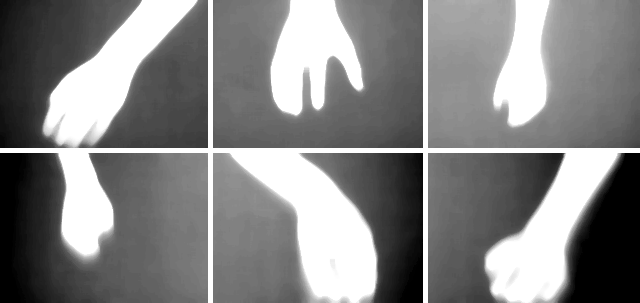
\includegraphics[width=0.8\textwidth]{images/empty_hand_correct.png}
  \caption{Příklady správně klasifikovaných snímků kategorie prázdná ruka}
  \label{fig:empty_hand_correct}
\end{figure} 

\begin{figure}[h]
  \centering
  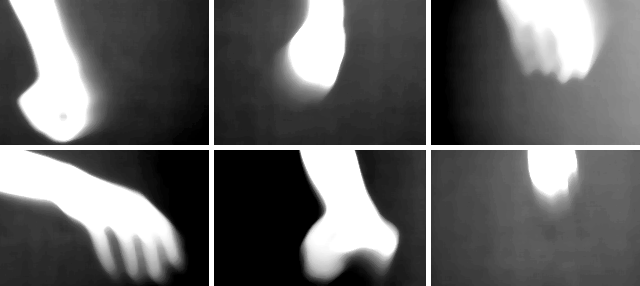
\includegraphics[width=0.8\textwidth]{images/empty_hand_wrong.png}
  \caption{Příklady klasifikovaných snímků jako ruka se zbožím, ale ve skutečnosti prázdná ruka}
  \label{fig:empty_hand_wrong}
\end{figure} 

\begin{figure}[h]
  \centering
  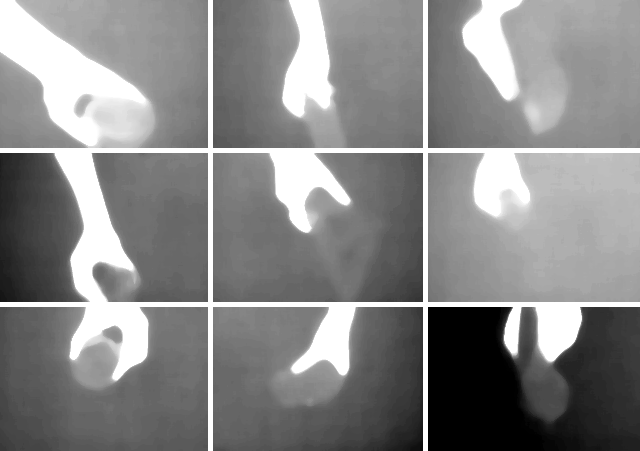
\includegraphics[width=0.8\textwidth]{images/hand_with_goods_correct.png}
  \caption{Příklady správně klasifikovaných snímků kategorie ruka se zbožím}
  \label{fig:hand_with_goods_correct}
\end{figure} 

\begin{figure}[h]
  \centering
  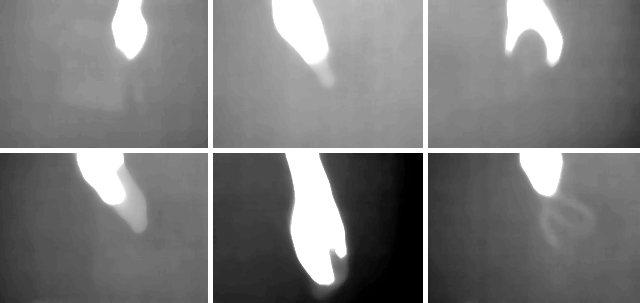
\includegraphics[width=0.8\textwidth]{images/hand_with_goods_wrong.png}
  \caption{Příklady klasifikovaných snímků jako prázdná ruka, ale ve skutečnosti ruka se zbožím}
  \label{fig:hand_with_goods_wrong}
\end{figure} 

	\subsection{Komentář ke klasifikaci snímků}
    Obecně by mělo být snadné detekovat ruku, protože na její teplotu se dá vždy spolehnout. Problém nastává při jejím rychlém pohybu, kdy pohybová neostrost zabrání jejímu správnému segmentování. Většina chybně klasifikovaných rukou jsou pohybově neostré snímky, případně snímky před kterými došlo ke změně pozadí, kdy se uložené pozadí ještě nestihlo adaptovat této změně.
    
    Z~chybně klasifikovaných snímků ruky se zbožím je zřejmé, že některé zboží mělo teplotu podobnou podlaze a na snímku je velmi obtížně rozlišitelné. Druhým případem je zboží, které je sice viditelné, ale má menší rozměry, takže po aplikaci morfologických operací již není rozpoznatelné.


\chapter{Implementované nástroje}
V~rámci práce bylo nutno vytvořit několik nástrojů, bez kterých by práce nemohla být splněna. Tato kapitola se tedy věnuje obecnému popisu nástrojů a implementačním detailům detekční aplikace. Ke každému nástroji jsou dostupné zdrojové kódy, které je možné nalézt na přiloženém paměťovém médiu a také v~online repozitářích \cite{ebusplayermod, thesisproject, flirimageviewer}. 

\section{Upravený eBUS Player}
Tento nástroj slouží ke konfiguraci a získávání dat z~termokamery. Proti jeho původní verzi byl modifikován přidáním síťové komunikace pro přenos dat. Původní aplikaci lze nalézt v~ukázkových kódech nástroje eBUS SDK. Zdrojový kód je psán v~jazyce C++ a je poměrně složitý k~pochopení (obsahuje přibližně 50 tříd), proto zde nebude více popisován.

\section{Aplikace s~detekčními algoritmy}
Tuto aplikaci lze považovat za hlavní a obsahuje implementaci algoritmů pro zpracování vstupního obrazu z~termokamery. Aplikace využívá algoritmy z~knihovny OpenCV. Obraz může být buď přijímán skrze soket rovnou z~kamery (pomocí modifikovaného eBUS Playeru), nebo načten z~předem definované složky.

Aplikace je koncipovaná tak, aby v~ní bylo možné algoritmy co nejlépe odladit. Obsahuje tlačítko pro pozastavení na vybraném snímku a pomocí uživatelského rozhraní je možné měnit parametry algoritmů a získat ihned náhled výsledku na konkrétním snímku. Důležitou vlastností je ukládání příchozích snímků ze soketu a poté možné jejich přehrávání s~předdefinovanou rychlostí. K~náhledu snímků slouží čtyři panely pro různé fáze zpracování. V~panelech se tedy objevuje: náhledový (předzpracovaný) snímek, snímek po odečtení pozadí, segmentovaná ruka, potencionální zboží. 

K~nastavování parametrů algoritmů slouží čtyři záložky, které jsou rozděleny do logických celků. Tyto nastavení je možné exportovat a importovat, využitý je formát XML.

	\subsection{Implementace}
    Cílem této práce není detailní popis návrhu a architektury, takže je uvedeno pouze pár základních informací, pro případné snadnější navázání na stávající řešení. Implementace je poměrně rozsáhlá a celá aplikace obsahuje přibližně 30 tříd, které jsou logicky rozděleny do několika balíků. 

    Celé uživatelské rozhraní zastřešuje ovladač MainController, který deleguje požadavky uživatele dál k~příslušným třídám. Tyto požadavky jsou nejčastěji na aktuálně využívaný obrazový detektor (AbstractDetector), aktuálně čtený zdroj (DataReciever) nebo na změnu nastavení parametrů algoritmu uložených v~paměti (Settings).    
    
	\subsubsection{AbstractDetector}
    Třída AbstractDetector je předek všech obrazový detektorů s~abstraktní metodou detect(). Potomci této třídy jsou celkem 3 a to: 
    \begin{description}
    \item [BackgroundDetector] slouží pro detekování snímků pozadí a jejich následné ukládání do definované složky.
    \item [MogDetector] vybraný a vyhodnocený algoritmus detekce pomocí odčítání pozadí uvedený v~\ref{section:background_substract_solution}.
    \item [EdgeDetector] algoritmus detekce využívající Cannyho hranový detektor uvedený v~\ref{section:edge_detection_solution}.
    \end{description}
     Pro detailnější informace o~struktuře těchto objektů je uveden diagram tříd \ref{fig:ea_class_detector}.

    \begin{figure}[h]
      \centering
      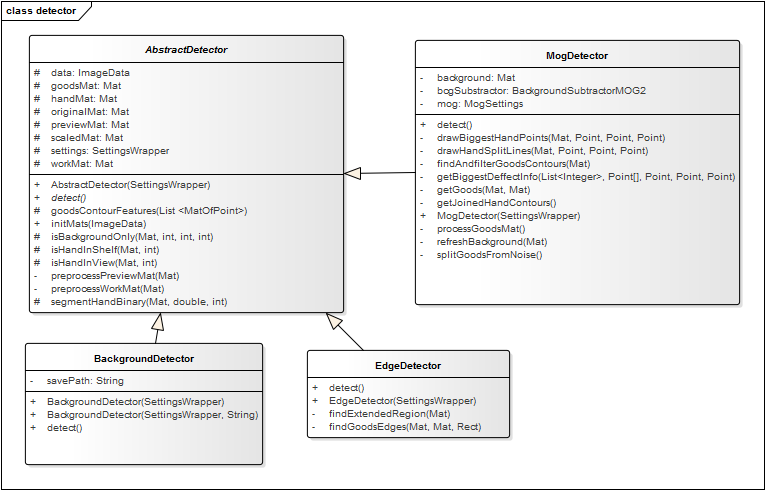
\includegraphics[width=1\textwidth]{images/ea_class_detector.png}
      \caption{Diagram tříd detekčních algoritmů}
      \label{fig:ea_class_detector}
    \end{figure} 
    
    \subsubsection{DataReciever}
    Pro příjem dat z~více zdrojů slouží abstraktní generická třída DataReciever. Jedním z~potomků této třídy je FlirDataReciever, který je využíván pro příjem dat z~termokamery a druhým potomkem je třída pro příjem z~webkamery nebo jiné USB kamery. Obě třídy implementují funkčnost ukládání a načtení snímků z~úložiště.

    \begin{figure}[h]
      \centering
      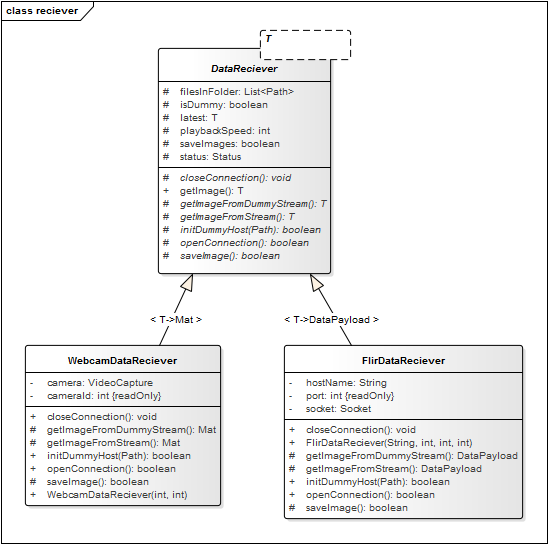
\includegraphics[width=1\textwidth]{images/ea_class_reciever.png}
      \caption{Diagram tříd zdrojů snímků}
      \label{fig:ea_class_reciever}
    \end{figure} 
    
    \subsubsection{Settings}
    V~paměti aplikace je uchováváno aktuální nastavení parametrů využívaných algoritmů. Tyto nastavení jsou rozděleny do čtyř skupin:
    \begin{description}
    \item [PreviewSettings] slouží k~aktivaci efektů algoritmů na náhledový snímek.
    \item [PreprocessingSettings] obsahuje jednotlivé parametry pro předzpracování obrazu před aplikací algoritmů.
    \item [MogSettings] jsou nastavení pro algoritmus odčítání pozadí.
    \item [EdgeDetectSettings] jsou nastavení parametrů algoritmu hranové detekce. Implementace těchto nastavení není dokončena.
    \end{description}
    Jednotlivé objekty nastavení jsou k~dispozici v~objektu SettingsWrapper, jehož instance je předávána všem detektorům. Všechna nastavení je možná exportovat do xml pomocí statické třídy SettingsManager.
    
    \begin{figure}[h]
      \centering
      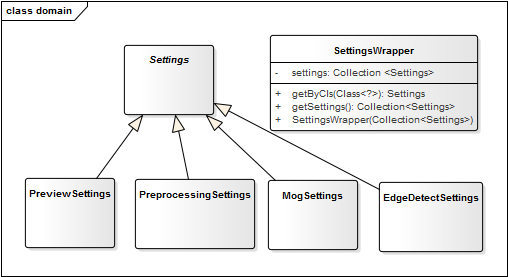
\includegraphics[width=1\textwidth]{images/ea_class_settings.png}
      \caption{Diagram tříd nastavení parametrů algoritmů}
      \label{fig:ea_settings}
    \end{figure} 

	\subsubsection{Práce s~obrazem}
    Poslední částí která stojí za zmínku je balíček image, jehož obsahem jsou dvě statické třídy MatOperations a ImageConvertor. Třída MatOperations je pomocná třída pro práci s~OpenCV maticemi, která a obsahuje volání knihovny, ale oproti běžnému volání nikdy nemodifikuje vstupní data. ImageConvertor obsahuje optimalizované metody pro převod mezi binárními daty, OpenCV maticemi a JavaFX obrázkem.

    \begin{figure}[h]
      \centering
      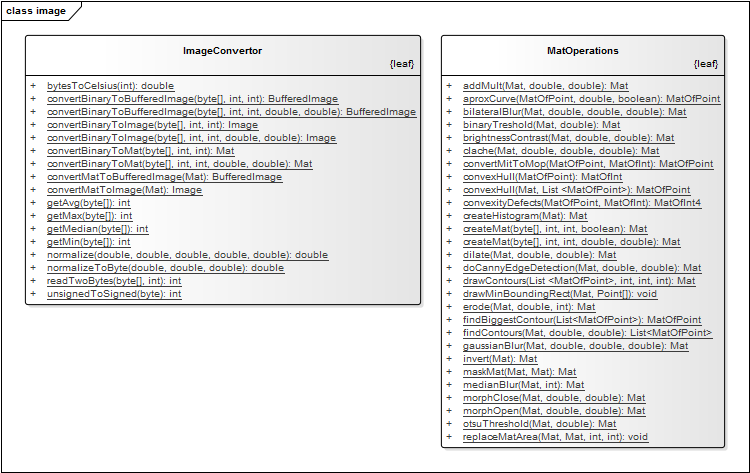
\includegraphics[width=1\textwidth]{images/ea_class_image.png}
      \caption{Diagram tříd baličku image}
      \label{fig:flir_binary_viewer}
    \end{figure} 


    \begin{figure}[h]
      \centering
      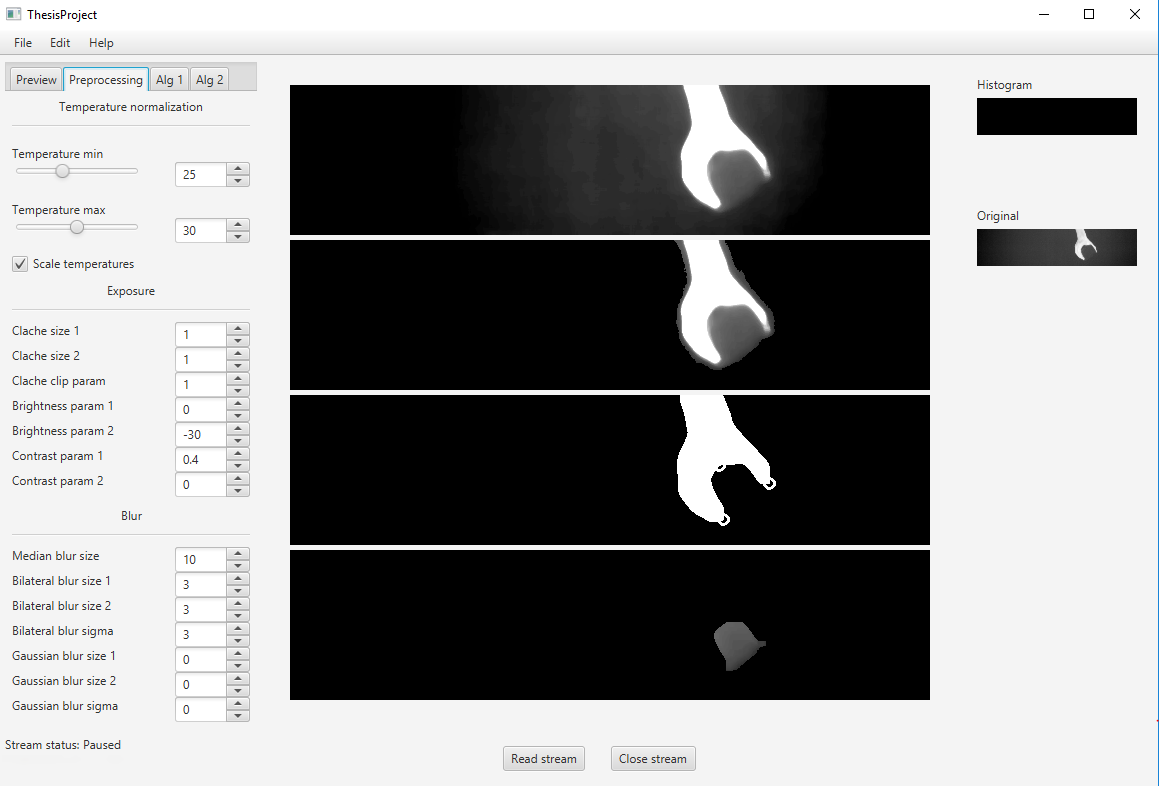
\includegraphics[width=1\textwidth]{images/main_app.png}
      \caption{Aplikace s~detekčními algoritmy}
      \label{fig:flir_binary_viewer}
    \end{figure} 
    
\clearpage

\section{Aplikace pro anotování snímků}
Pro potřeby vyhodnocování bylo nutné jednotlivé snímky rozdělit do skupin. K~tomu byl vytvořen tento nástroj, který lze snadno ovládat pomocí klávesnice a tím rychle rozřazovat jednotlivé snímky. 

Přesouvání mezi jednotlivými snímky probíhá pomocí klávesnicových šipek a přesunutí snímku do předem definované složky pomocí čísla 1-4 v~závislosti na kategorii. Snímky je též možné vyhledávat pomocí textového pole a pomocí klávesy D odstraňovat.

V~implementaci nejsou žádné složitosti. Aplikace se skládá pouze z~jednoho ovladače (MainController), který deleguje požadavky uživatelského rozhraní. Soubory jsou udržovány v~objektu InMemoryFiles, který snímky v~paměti spravuje a poskytuje je zpět do GUI podle nutnosti. Všechny metody pro převod binárního souboru na snímek poskytuje statická třída ImageConversions.

\begin{figure}[h]
  \centering
  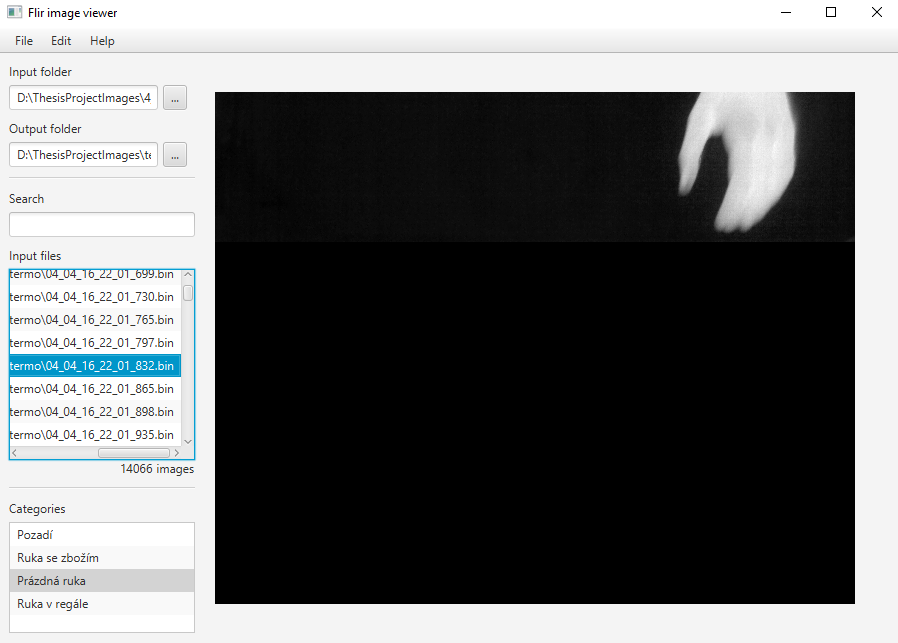
\includegraphics[width=1\textwidth]{images/flir_binary_viewer.png}
  \caption{Aplikace pro anotování snímků}
  \label{fig:flir_binary_viewer}
\end{figure} 
\chapter{Zhodnocení}
Práce se nakonec ukázala o~něco složitější, než se na začátku zdálo. Přes všechny možné nástrahy od poruchy původní kamery až nestabilitu obrazu se nakonec povedlo najít rozumné řešení, které vzhledem k~dostupným prostředkům poskytuje poměrně slušné výsledky. 

\section{Využitá technika}
Během práce se bohužel vyskytla závada na původní kameře (25 mm) a bylo nutné využít záložní kameru (13 mm) s~jinou ohniskovou vzdáleností a horší snímkovací frekvencí. Tato kamera (13 mm) měla širší úhel záběru, takže ji bylo nutné více přiblížit k~regálu. Původní kamera (25 mm) byla pro tuto úlohu vhodnější, protože delší ohnisková vzdálenost přispěla k~tomu, že kolem regálu nebyl snímán zbytečně velký prostor. Jedinou nevýhodou delší ohniskové vzdálenosti je, že v~snímané oblasti regálu byla menší hloubka ostrosti než při snímání s~kamerou (13 mm) s~širší ohniskovou vzdáleností. 

7.5 snímků za vteřinu u~náhradní kamery (13 mm) je obecně velmi málo, ale i přesto se dalo při rozšíření oblasti zájmu dosáhnout poměrně slušných výsledků. V~případě že by bylo vyhodnocování provedeno na funkční kameře (25 mm), byly by výsledky lepší, protože díky vyšší snímkovací frekvenci se algoritmus zvládne rychleji adaptovat na změnu prostředí. Dostačující by byla i kamera se snímkovací frekvencí 15 Hz.

\section{Navržené řešení}
Finální navržený algoritmus se i přes nestabilitu obrazu z~kamery jeví, proti ostatním navrženým řešením, jako robustní. Je schopný se poměrně rychle adaptovat na změny prostředí, která vznikají v~malé míře při postupném zahřívání detektoru a ve velké míře při kalibrací NUC.

Stávající řešení by bylo možné ještě různými způsoby vylepšovat, ale je nutné se zamyslet nad tím, zda se jedná opravdu o~nejlepší možný způsob řešení. Vylepšení, které by určitě pomohlo je zaměřit se na stabilizování snímané scény. Pro zlepšení stability scény by bylo nutné implementovat algoritmus, pro co nejlepší stanovení hodnot $min$ a $max$ použitých při normalizaci snímku. V~tuto chvíli jsou tyto hodnoty nastavovány ručně. Ruční nastavení poskytuje mnohem lepší výsledky než normalizace pomocí nalezení minimální a maximální teploty v~snímku. 

Vylepšení, které by přineslo největší přínos je zaměřit se na více obrazových zdrojů. Termokamera se hodí perfektně pro segmentaci ruky, ale segmentovat pomocí termokamery předměty, které mají velmi podobné teploty jako pozadí, se ukázalo jako velmi obtížné. V~\ref{section:combining_rgb_and_thermal} bylo navrženo řešení využívající viditelný a termovizní snímek, ale nakonec nebylo implementováno kvůli vzniklým problémům se synchronizací.

\section{Implementace řešení}
Vytvořená aplikace s~algoritmy detekce slouží též jako klient pro příjem snímků z~aplikace eBUS Player. Mezi přenosem dat těchto dvou aplikací vzniká jen minimální zpoždění a je možné nad daty pracovat téměř v~reálném čase. Toto bylo bráno v~potaz při implementaci jednotlivých metod, které jsou maximálně optimalizovány. Případným rozšířením o~klasifikátor lze tedy ihned vyhodnocovat. Aplikace je též připravena na příjem více datových zdrojů, jako je například obraz z~RGB kamery.

Aplikace má vytvořené uživatelské rozhraní s~velmi dobrou správou nastavení parametrů algoritmů. Návrh aplikace je smysluplný, podstatné části jsou komentovány a je tedy snadné ji dále rozšiřovat.

\section{Výsledky řešení}
Výsledky byly lehce ovlivněny tím, že mezi manipulací se zbožím nebyly nechávány dostatečné přestávky. Tyto nedostatečné pauzy způsobily, že při změně obrazového prostředí (NUC, teplotní drift) nebyl získán dostatečný počet snímků pro adaptaci uloženého pozadí. To způsobuje zhoršení výsledků operace odečtení pozadí, která na scéně zahrne větší oblast popředí než reálně existuje a prázdná ruka pak může být klasifikována jako ruka se zbožím. Tento problém byl bohužel zjištěn až v~poslední fázi při vyhodnocování, kdy už byla nasnímána všechna data.

Klasifikace probíhala pomocí nástroje RapidMiner a bylo vyzkoušeno mnoho klasifikátorů a různých nastavení. Ke klasifikaci bylo využito 20 atributů zaměřených na vlastnosti kontur. V~případě že by byl k~dispozici stabilní obrazový výstup, dávalo by smysl přidat atributy zaměřující se na vlastnosti obrazu. Přidání dalších užitečných atributů by výsledky klasifikace zlepšilo. 

K~dispozici byl poměrně skromný data set s~přibližně 1200 anotovanými snímky. Při využití většího datasetu by byl vytvořen robustnější model. Klasifikovány byly snímky pouze z~kamery (13 mm).

\section{Budoucí využití}
V~budoucnu by bylo možné téma ještě dále rozvíjet, protože vylepšení ještě nejsou zdaleka vyčerpány. Jedno z~budoucích témat by mohlo být například detekce pomocí termokamery a kamery Microsoft Kinect s~využitím více obrazových zdrojů. Kombinací obrazových zdrojů by bylo možné stávající řešení zdokonalit, protože každé spektrum přináší o~snímaném obrazu nové informace. Bohužel kombinace obrazů z~různých zdrojů je velmi obtížné téma a přináší s~sebou spoustu dalších komplikací. Toto téma by se tedy hodilo převážně pro diplomovou práci.
\begin{conclusion}
Cílem práce bylo vytvoření algoritmu pro detekci zboží v~ruce zákazníka pomocí snímků z~termokamery. K~tomu bylo nutné se seznámit s~technologií termokamer a oborem termografie. V~rešeršní části byly nabyty znalosti pro návrh vlastního řešení, které následně bylo s~jejich pomocí implementováno. Na řešení úlohy bylo nahlíženo různými způsoby a byly navrhnuty celkem čtyři různé algoritmy. Implementovány jsou dva z~nich a jsou k~nalezení v~přiložené aplikaci. Vytvořená aplikace poskytuje uživatelské rozhraní pro snadnou práci s~daty a konfiguraci podstatných parametrů aplikovaných algoritmů. Pro vyhodnocení výsledků práce je použito řešení s~využitím algoritmu dynamického odčítání pozadí. K~vyhodnocování se využívají vlastnoručně naměřená data z~Laboratoře pro zpracování obrazu na FIT ČVUT s~pomocí termokamery FLIR A65 umístěnou nad regálem. Na základě výsledků algoritmu je provedena diskuze, kde jsou uvedeny souhrnné informace o~finálním řešení a jeho možné budoucí vylepšení.

    

\end{conclusion}

\bibliographystyle{csn690}
\bibliography{ref}

\appendix

\chapter{Seznam použitých zkratek}
% \printglossaries
\begin{description}
	\item[AIA] Automated Imaging Association
	\item[BSD] Berkeley Software Distribution
    \item[CIE] International Commission on Illumination

    \item[EMVA] European Machine Vision Association
    \item[FPS] Frames per second
    \item[FPA] Focal Plane Array
    \item[GBT] Gradient boosted trees
    \item[GUI] Graphical user interface
    \item[HMM] Hidden Markov Model

	
    \item[IR] Infrared

	\item[MOG] Mixture of gaussians
    \item[NUC] Non-Uniformity Correction 

	\item[PoE] Power over Ethernet
    \item[UDP] User Datagram Protocol

	\item[SVM] Support vector machines
    
	\item[RGB] Red, Green, Blue
	\item[UV] Ultraviolet
	\item[XML] Extensible markup language
\end{description}

\chapter{Obsah přiloženého média}

%upravte podle skutecnosti

\begin{figure}
	\dirtree{%
		.1 readme.txt\DTcomment{stručný popis obsahu přiloženého média}.
		.1 src.
		.2 impl\DTcomment{adresář s~implementovanými nástroji}.
        .3 eBUSPlayer\DTcomment{zdrojové kódy upravené aplikace eBUS Player}.
        .3 ThesisProject\DTcomment{zdrojové kódy hlavní aplikace s~algoritmy}.
        .3 FlirBinaryViewer\DTcomment{zdrojové kódy nástroje pro prohlížení a anotování snímků}.
		.2 thesis\DTcomment{zdrojová forma práce ve formátu \LaTeX{}}.
		.1 text\DTcomment{text práce}.
		.2 thesis.pdf\DTcomment{text práce ve formátu PDF}.
        .1 image\_examples\DTcomment{několik ukázkových snímků z~termokamery}.
        .1 dataset\DTcomment{složka s~vyhodnocovaným datasetem}.
	}
\end{figure}

\end{document}
